% !Mode:: "TeX:UTF-8"

\clearemptydoublepage
\chapter[景深对 HAADF-STEM 原子分辨率三维重构的影响]{景深对 HAADF-STEM 原子分辨率\\三维重构的影响}
\section{引言}
3DET 是通过物体沿不同方向的投影来重构物体内部三维结构信息的方法~\cite{Frank2006,Kubel2005},在利用透射电镜研究材料三维微观结构方面有广泛的应用。HAADF-STEM 信号来源于高角度的散射电子,这些电子主要与样品中的原子核发生卢瑟福散射,散射角度主要受到样品中原子序数的影响。因此,其信号强度在一级近似下与样品内原子的原子序数呈线性关系~\cite{Midgley2003}。一般认为 HAADF-STEM 像属于质厚衬度成像,即为样品内部结构的线性投影。因此,HAADF-STEM 像被广泛地应用于 3DET 之中。

随着像差校正 TEM 设备和技术突飞猛进的发展,STEM 能够产生的会聚电子束斑越来越小,从而使 HAADF-STEM 像的二维空间分辨率能够达到 1 埃以下,可以清晰地分辨原子~\cite{Haider1998,Hosokawa2013}。近年来,利用原子分辨率 HAADF-STEM 倾转系列像进行原子分辨率三维重构的工作被陆续报道~\cite{Miao2016,Xu2015,Scott2012,VanAert2011,Lu2015,Azubel2014},对理解材宏观料性能与其微观结构之间的关系具有重要指导意义。然而,原子分辨率的三维重构依然是一项具有挑战性的工作,其难点不仅仅在于实验数据的收集,还在于对 STEM 倾转系列像 3DET 技术缺乏透彻的理论理解。当 STEM 的电子束斑的横向分辨率达到埃量级及以下时,其纵向景深也会减小至纳米量级。此时,HAADF-STEM 像将不再是整个样品内部结构的线性投影,而会转变为样品内部某一深度的光学层析~\cite{Xin2009,Ishikawa2015,Yang2015,Borisevich2006-1,Bosch2020},不再符合倾转系列三维重构对线性投影的要求。因此,在已有的理论模拟和实验结果中,样品的厚度均小于电子束的景深~\cite{Xu2015,VanAert2011,Aveyard2016}。Robert Hovden 等~\cite{Hovden2014}认为当景深小于样品的厚度时,倾转系列三维重构将不可实现。为了突破样品大小的限制,他们提出结合系列欠焦图像来获得足够的样品信息以供三维重构。无独有偶,C. Jacobsen~\cite{Jacobsen2018}提出利用 ptychography 技术,在每个投影方向收集多个厚度层的投影信息来弥补样品信息的不足。然而到目前为止,景深对原子分辨率三维重构的影响尚没有太多研究,人们对原子分辨率 3DET 在理论上的认识还存在不足。

本章通过多层法 STEM 图像模拟和 3DET 重构,研究了纳米尺度景深下原子分辨率 3DET 的可行性,并讨论了景深对原子分辨率 3DET 的影响。结果表明,当景深小于样品厚度时,三维重构技术只能正确重构样品中的局部区域。该区域的大小与入射电子束景深呈正相关,位置与入射束的欠焦量有关。另外,研究还发现实际正确重构的区域相对于电子束名义聚焦位置偏上,即存在提前聚焦现象。

\section{图像模拟与三维重构}
\subsection{HAADF-STEM 倾转系列像的多层法模拟}
HAADF-STEM 图像的多层法模拟计算始于二维的入射会聚电子束束斑波函数方程 $\psi_0$,它的具体表达式如下~\cite{Kirkland2011,Aveyard2016,Tanaka1999}:
\begin{equation}
\psi_0(\boldsymbol{r}) = A_pFT^{-1}\left\{\exp\left[-i\chi(\boldsymbol{k})\right]\cdot A(\boldsymbol{k})\right\}
\end{equation}
\begin{equation}
A(\boldsymbol{k})=\left\{ \begin{array}{cc} 0, &|\boldsymbol{k}|>\theta /\lambda \\ 1, &|\boldsymbol{k}|\leq \theta /\lambda 
\end{array} \right.
\end{equation}
此处,$\boldsymbol{r}$ 为二维实空间坐标,$A_p$ 是归一化因子,$FT^{-1}$ 表示二维反傅里叶变换, $\boldsymbol{k}$ 是二维倒空间坐标,$A$ 表示聚光镜光阑,$\theta$ 是聚光镜光阑半角,$\lambda$ 是电子束的波长,$\chi$ 表示像差方程。与第 1.2.3 条中的公式(1.11)不尽相同,本研究忽略了除欠焦量以外的像差,因此 $\chi(\boldsymbol{k})= \pi\lambda\Delta f\boldsymbol{k}^2$,$\Delta f$ 是欠焦量。通过调节 $\Delta f$ 可以改变电子束在 $z$ 方向上的聚焦位置。

电子束斑入射到样品某一位置时,与样品的交互作用通过多层法模拟。多层法模拟的方法已经在第 1.2.4.1 款中介绍,这里不再赘述。

由于 HAADF 探测器位于背焦面处,即电子衍射空间,因此末层的出射波函数将通过傅里叶变换得到倒易空间波函数 $\Psi_{ext}(\boldsymbol{k})$,并与探测器函数相作用得到最终的图像散射强度。此外,本研究中以冷冻声子模型~\cite{Wang1998,Alania2018}计算热漫散射~\cite{Hillyard1995} 对图像的影响。

\subsection{景深}
景深,也被称作垂直分辨率,它描述了电子束斑在深度($z$)方向上所能影响的范围,如 P.D. Nellist 等~\cite{Nellist2007}的论文中定义景深是电子束斑在光轴上保持 1/2 最大强度的距离。参考多篇论文,景深的具体表达式如下:
\begin{equation}
\Delta z=\alpha \frac{\lambda}{\theta^2}
\end{equation}
此处,根据不同的定义,$\alpha=1 \sim3.5$~\cite{Ishikawa2015,Nellist2007,Born1980,Lee2013}。从上式可知,电子束的加速电压是影响景深的一个重要因素,高电压获得短波长的电子束的景深较小。另一方面,聚光镜光阑的尺寸决定会聚半角 $\theta$ 的大小,所以它也是影响景深的另一个重要因素。在实际的电镜使用中,聚光镜光阑的作用是阻挡电子束中像差较大的部分,只留下中间像差较小的部分,以获得均匀对称的电子束。所以实际使用的聚光镜光阑的尺寸与电子束中的残余像差有关。在本研究的模拟测试中,为了简化对比,忽略了实际情形中像差与聚光镜光阑的关系,将欠焦量以外的所有像差假设为 “0”,直接根据公式(3.2),模拟不同会聚半角的电子束。不过,根据 Varat Intaraprasonk 等~\cite{Intaraprasonk2008}介绍的优化最佳光阑尺寸的方法,也可以在模拟中考虑像差与聚光镜光阑的关系,得到符合实际的具有像差的入射电子束。

图 3.1 展示了不同加速电压和会聚半角的模拟电子束束斑。图 3.1a 中的会聚半角仅 10 mrad,代表一般的非球差校正电镜的束斑,可见束斑的尺寸非常大,根据公式(3.3)计算得其在加速电压为 200 kV 时的景深为 $25.1 \sim 87.9$ nm。图 3.1b 代表了一般的球差校正电镜的束斑,会聚半角为 30 mrad。它的尺寸相对于会聚半角为 10 mrad 时明显变小,其对应的景深为 $2.8 \sim 9.8$ nm。图 3.1c 代表了先进的球差校正电镜中的束斑,会聚半角进一步增大为 50 mrad,此时景深为 $1.0 \sim 3.5$ nm。作为对比,将其中的加速电压降低至 100 kV 后,如图 3.1d 所示,束斑尺寸相应变大。

\begin{figure}[H]
	\vspace{\baselineskip}
	\centering
	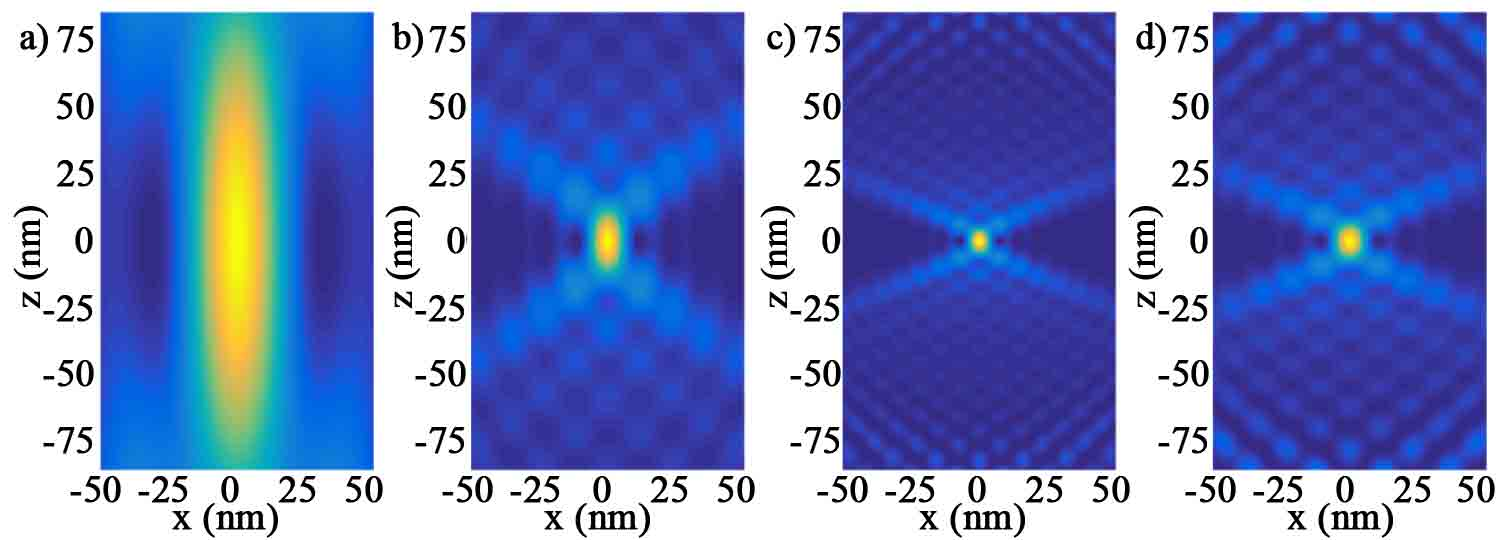
\includegraphics[width=0.9\textwidth]{../4.11/411}
	\caption{不同参数的电子束斑}\label{fig:413}
	\song\tuzhu{a) 加速电压 200 kV,会聚半角 10 mrad;b)  加速电压 200 kV,会聚半角 30 mrad;c)  加速电压 $\textnormal{200 kV}$,会聚半角 50 mrad;d) 加速电压 100 kV,会聚半角 50 mrad}
\end{figure}

\subsection{倾转系列三维重构}
在本研究中,倾转系列三维重构是根据 D. Wolf 等~\cite{Wolf2014} 的论文中介绍的同时迭代重构技术实现的。这个技术的核心算法如下所示:
\begin{equation}
f_t=f_{t-1}+\omega\mathcal{R}^{-1}\left(\hat{f}^{exp}-\mathcal{R}f_{t-1}\right)
\end{equation}
其中,$f_t$ 和 $f_{t-1}$ 是第 $t$ 和 $t-1$ 次重构的结果,$\mathcal{R}$ 和 $\mathcal{R}^{-1}$ 分别表示拉登变换和反拉登变换,$\hat{f}^{exp}$是实验倾转系列像,$\omega$ 是收敛因子。该算法通过本实验室编写的代码实现,对模拟的 HAADF-STEM 倾转系列像进行重构。

\subsection{计算模型与参数}
本章利用图像模拟生成样品沿不同方向的 STEM 图像,并利用这些图像进行三维重构,讨论景深对原子分辨率三维重构的影响。图  3.2 展示了用于计算的样品模型。为了避免通道效应~\cite{WangA2010,Sinkler1999}对三维重构带来的假象,该模型的原子在 $x-z$ 面内处于无序状态,如图 3.2a 所示。另外,由于样品 $x-z$ 方向被真空层包裹,由图像模拟的周期性重复假设所引起的环绕效应~\cite{Kirkland2010}可以被忽略。该无序原子模型的总尺寸是 $15 \textnormal{ nm} \times 15 \textnormal{ nm} \times 2.4 \textnormal{ nm}$,中间样品的尺寸是 10 nm $\times$ 10 nm $\times$ 2.4 nm(下文中的尺寸均指中间样品的尺寸)。在图像模拟测试中,电子束沿 $z$ 轴入射。由于块体三维重构可视为多个二维重构图像的有序堆叠,因此本章只重构二维图像中的其中一层,如图 3.2b,c 所示。从图 3.2b 可以看出,样品中各原子均严格处于一个 $x-z$ 平面内,这便于对重构的结果进行分析。图 3.2c 展示了该原子层的原子结构图。从图中可以看出,样品在 $x-z$ 面内的周期性被破坏,因此模拟过程中不存在通道效应。

\begin{figure}[H]
	\vspace{\baselineskip}
	\centering
	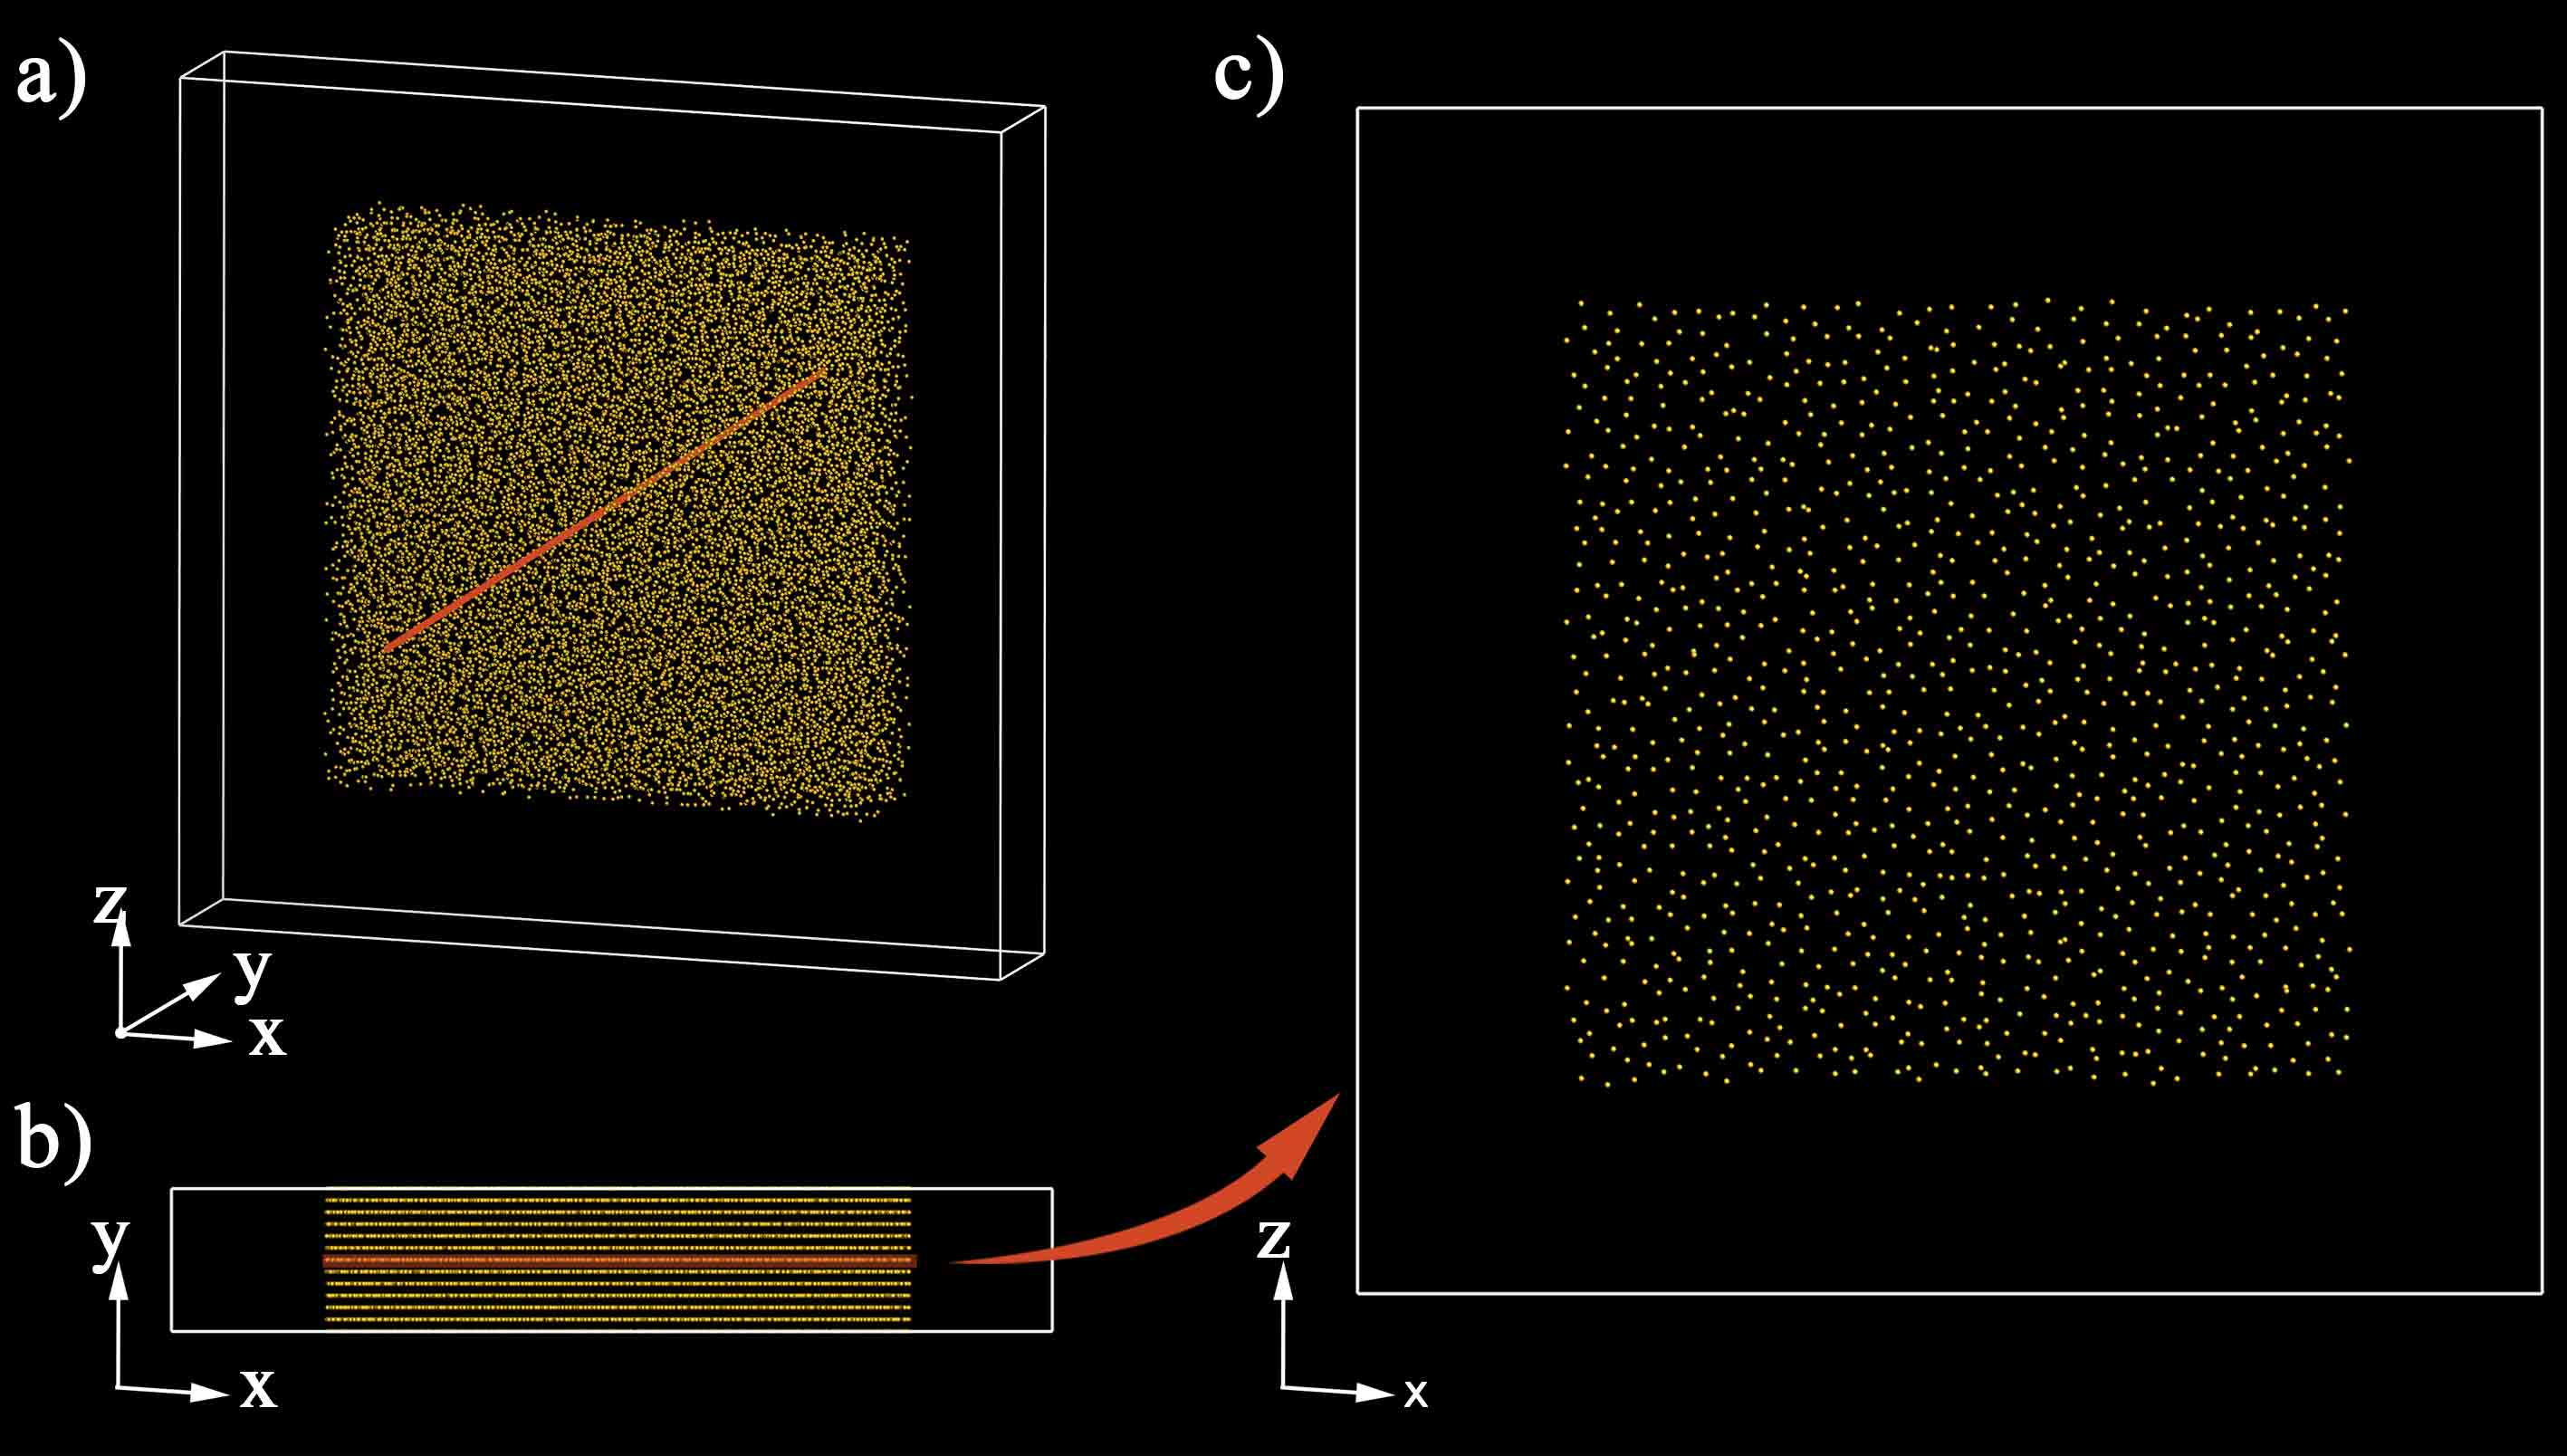
\includegraphics[width=0.85\textwidth]{../4.1/41}
	\caption{用于图像模拟的三维模型}\label{fig:41}
	\song\tuzhu{a) 原子模型侧视图,图中橙线表示倾转轴;b) 原子模型顶视图,橙线代表中间原子层;c) 图 b 中橙线所标志的中间原子层的正视图}
\end{figure}

在多层法模拟中,电子束斑的采样为 $512\times 512$ 像素,对应实际尺寸 2.4 nm $\times$ 2.4 nm,在倒空间中足以完整计算 267.7 mrad 之内的信息。欠焦量以外的像差如前所述均设置为“0”。HAADF 探测器收集角为 $90\sim230$ mrad,冷冻声子模型声子态为 16。会聚半角、加速电压、欠焦量、模型的厚度和原子序数是本研究的对比参数。多层法像模拟通过本实验室编写的代码实现,其中使用了图形处理单元计算加速技术~\cite{MWQ2018}。倾转系列像的倾转角为 -90º 至 +89º,倾转间隔 1º。

此外,为了对比,本章还用同样的方法建立了尺寸为 5 nm $\times$ 5 nm $\times$ 2.4 nm 和 2.4 nm $\times$ 2.4 nm $\times$ 2.4 nm(不包含真空层的尺寸)的无序原子模型。

\section{结果与分析}
\subsection{局部区域重构现象}
图 3.3 是将会聚半角为 50 mrad,加速电压为 200 kV (此时的景深为 $1.0 \sim 3.5$  nm)的入射束,聚焦到尺寸为 10 nm $\times$ 10 nm $\times$ 2.4 nm 的铝原子模型内 1/4、1/2 和 3/4 深度时的重构结果。从图 3.3a-c 可知,当电子束斑的景深小于样品的厚度时,样品局部区域的原子位置仍可被清晰地重构,且该正确重构的区域随电子束斑聚焦的位置而移动。

\begin{figure}[H]
	\vspace{\baselineskip}
	\centering
	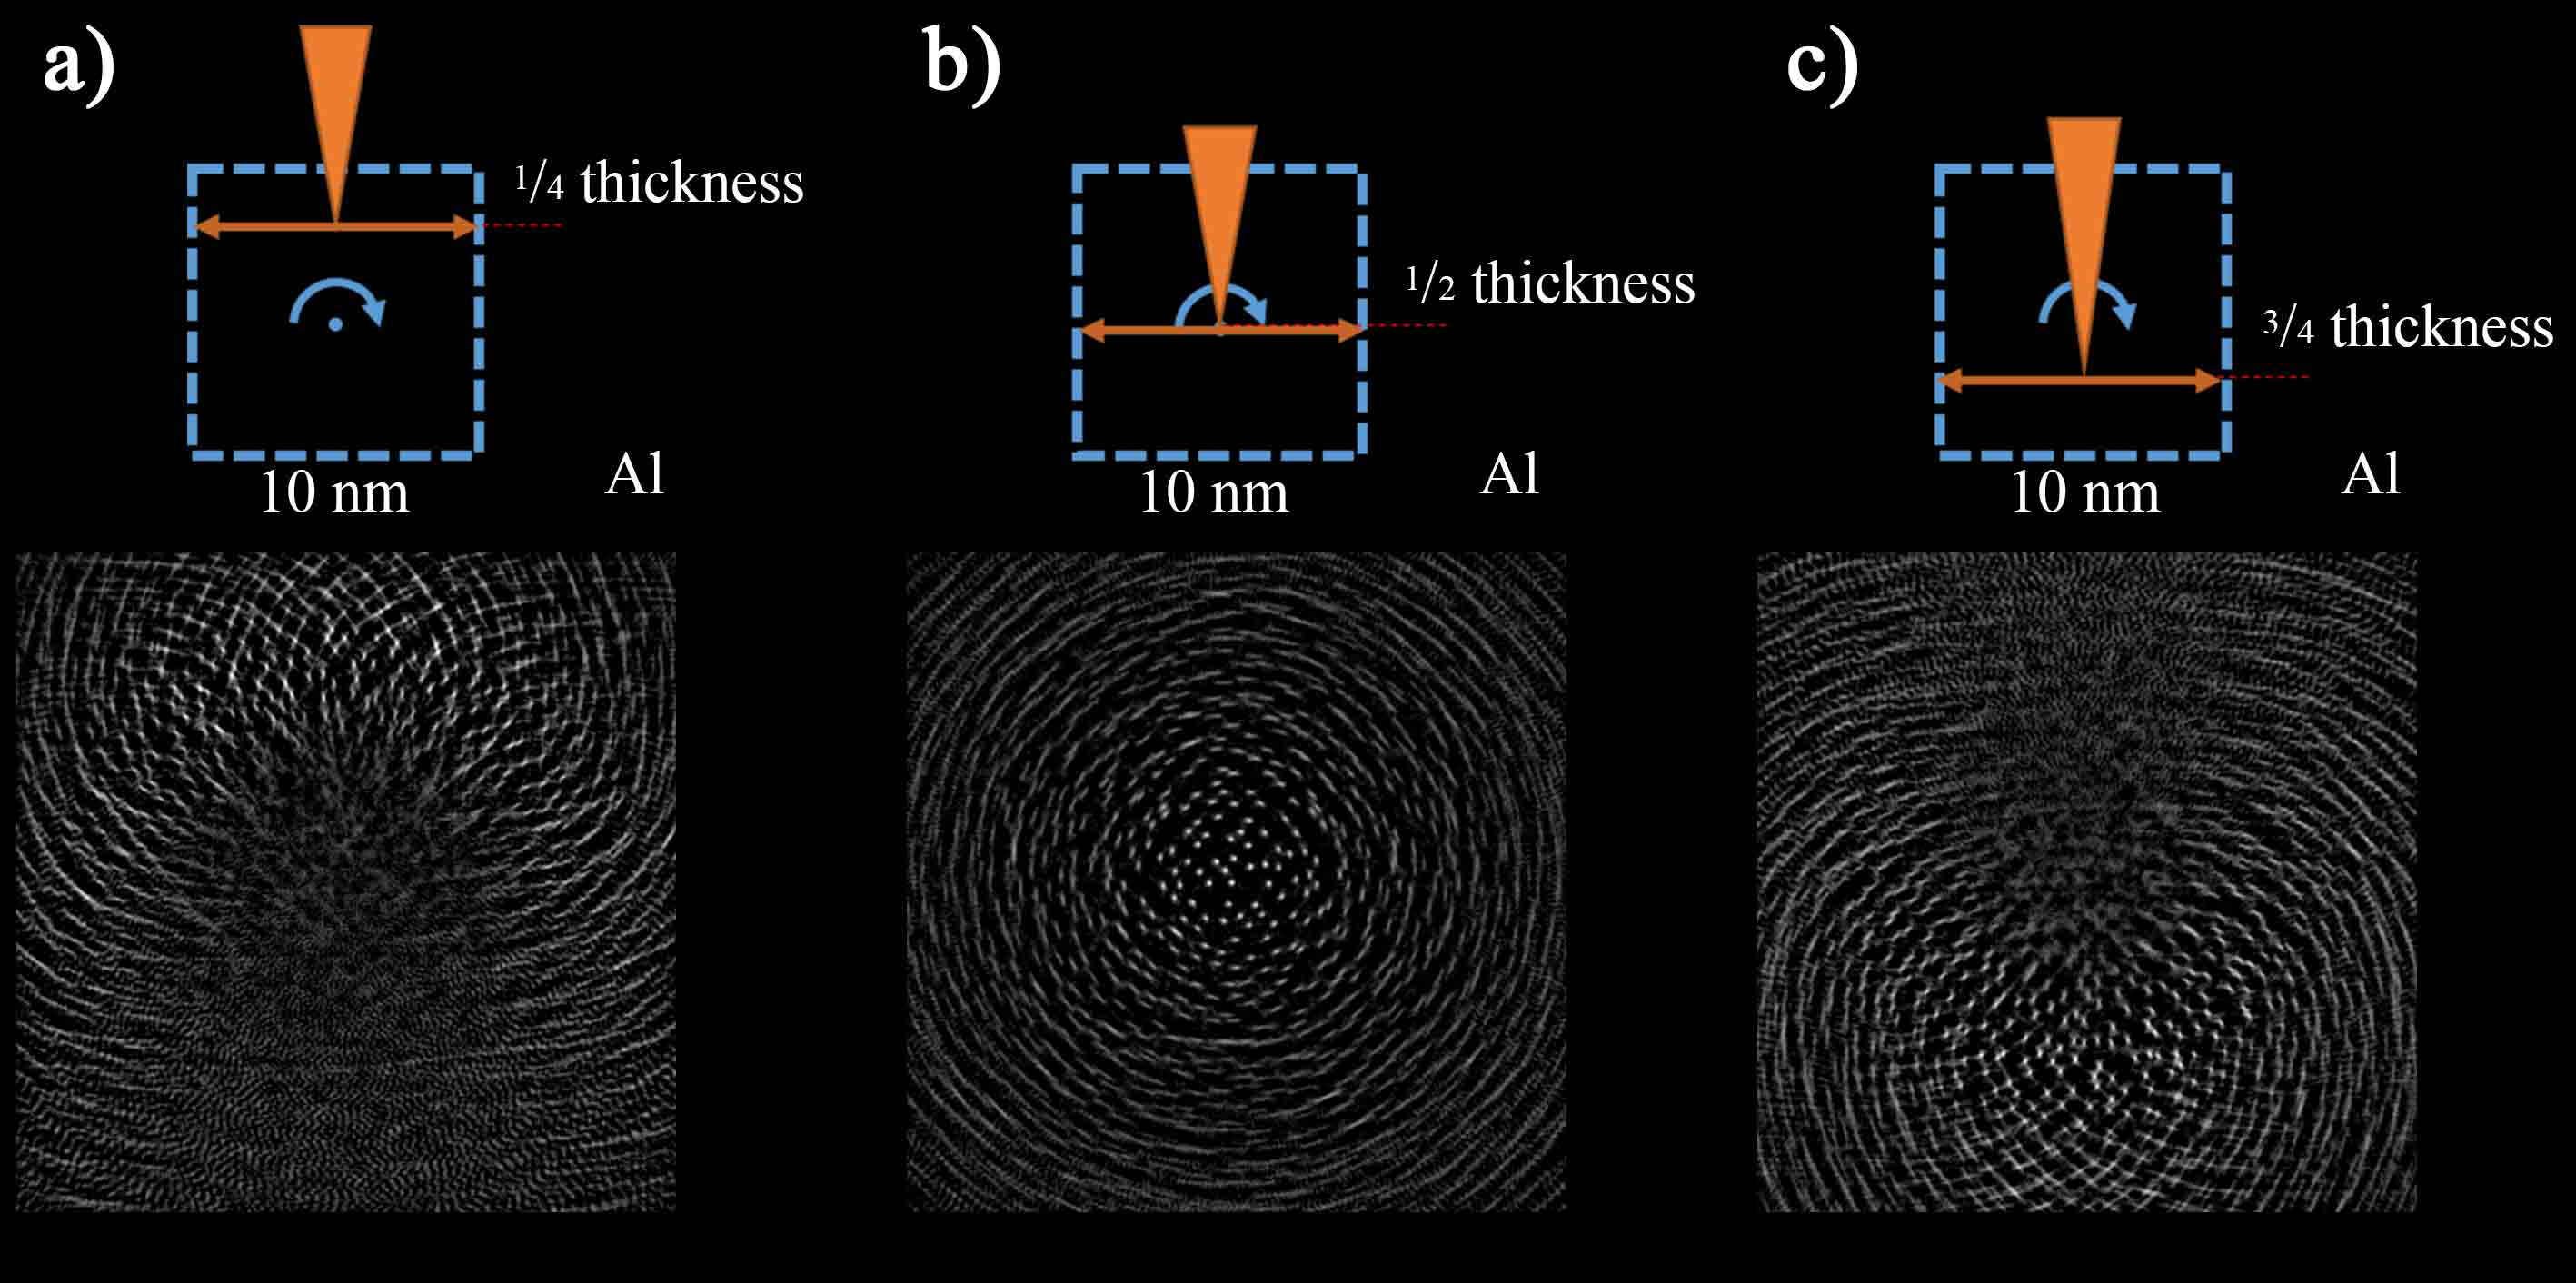
\includegraphics[width=0.85\textwidth]{../4.2/42}
	\caption{尺寸为 10 nm $\times$ 10 nm $\times$ 2.4 nm 的铝原子模型的重构结果}\label{fig:42}
	\song\tuzhu{电子束斑分别被聚焦到深度为:a) 1/4 样品厚度;b) 1/2 样品厚度;c) 3/4 样品厚度的位置;电子束的会聚半角均为 50 mrad,加速电压是 200 kV}
\end{figure}

图 3.4 是将会聚半角为 50 mrad,加速电压为 200 kV(此时的景深为 $1\sim3.5$ nm)的电子束会聚至尺寸分别为 10 nm $\times$ 10 nm $\times$ 2.4 nm,5 nm $\times$ 5 nm $\times$ 2.4 nm 和 2.4 nm $\times$ 2.4 nm $\times$ 2.4 nm 的铝原子模型内 1/2 深度时的重构结果。在图 3.4a-c中,红色正方形虚线框对应的边长为 2.4 nm,黄色正方形虚线框对应的边长为 5 nm。通过对比可以明显地看出,尽管模型大小不同,在相同的成像条件下,被正确重构出原子位置的区域的尺寸,在三种情况下均接近 2.4 nm。

\begin{figure}[H]
	\vspace{\baselineskip}
	\centering
	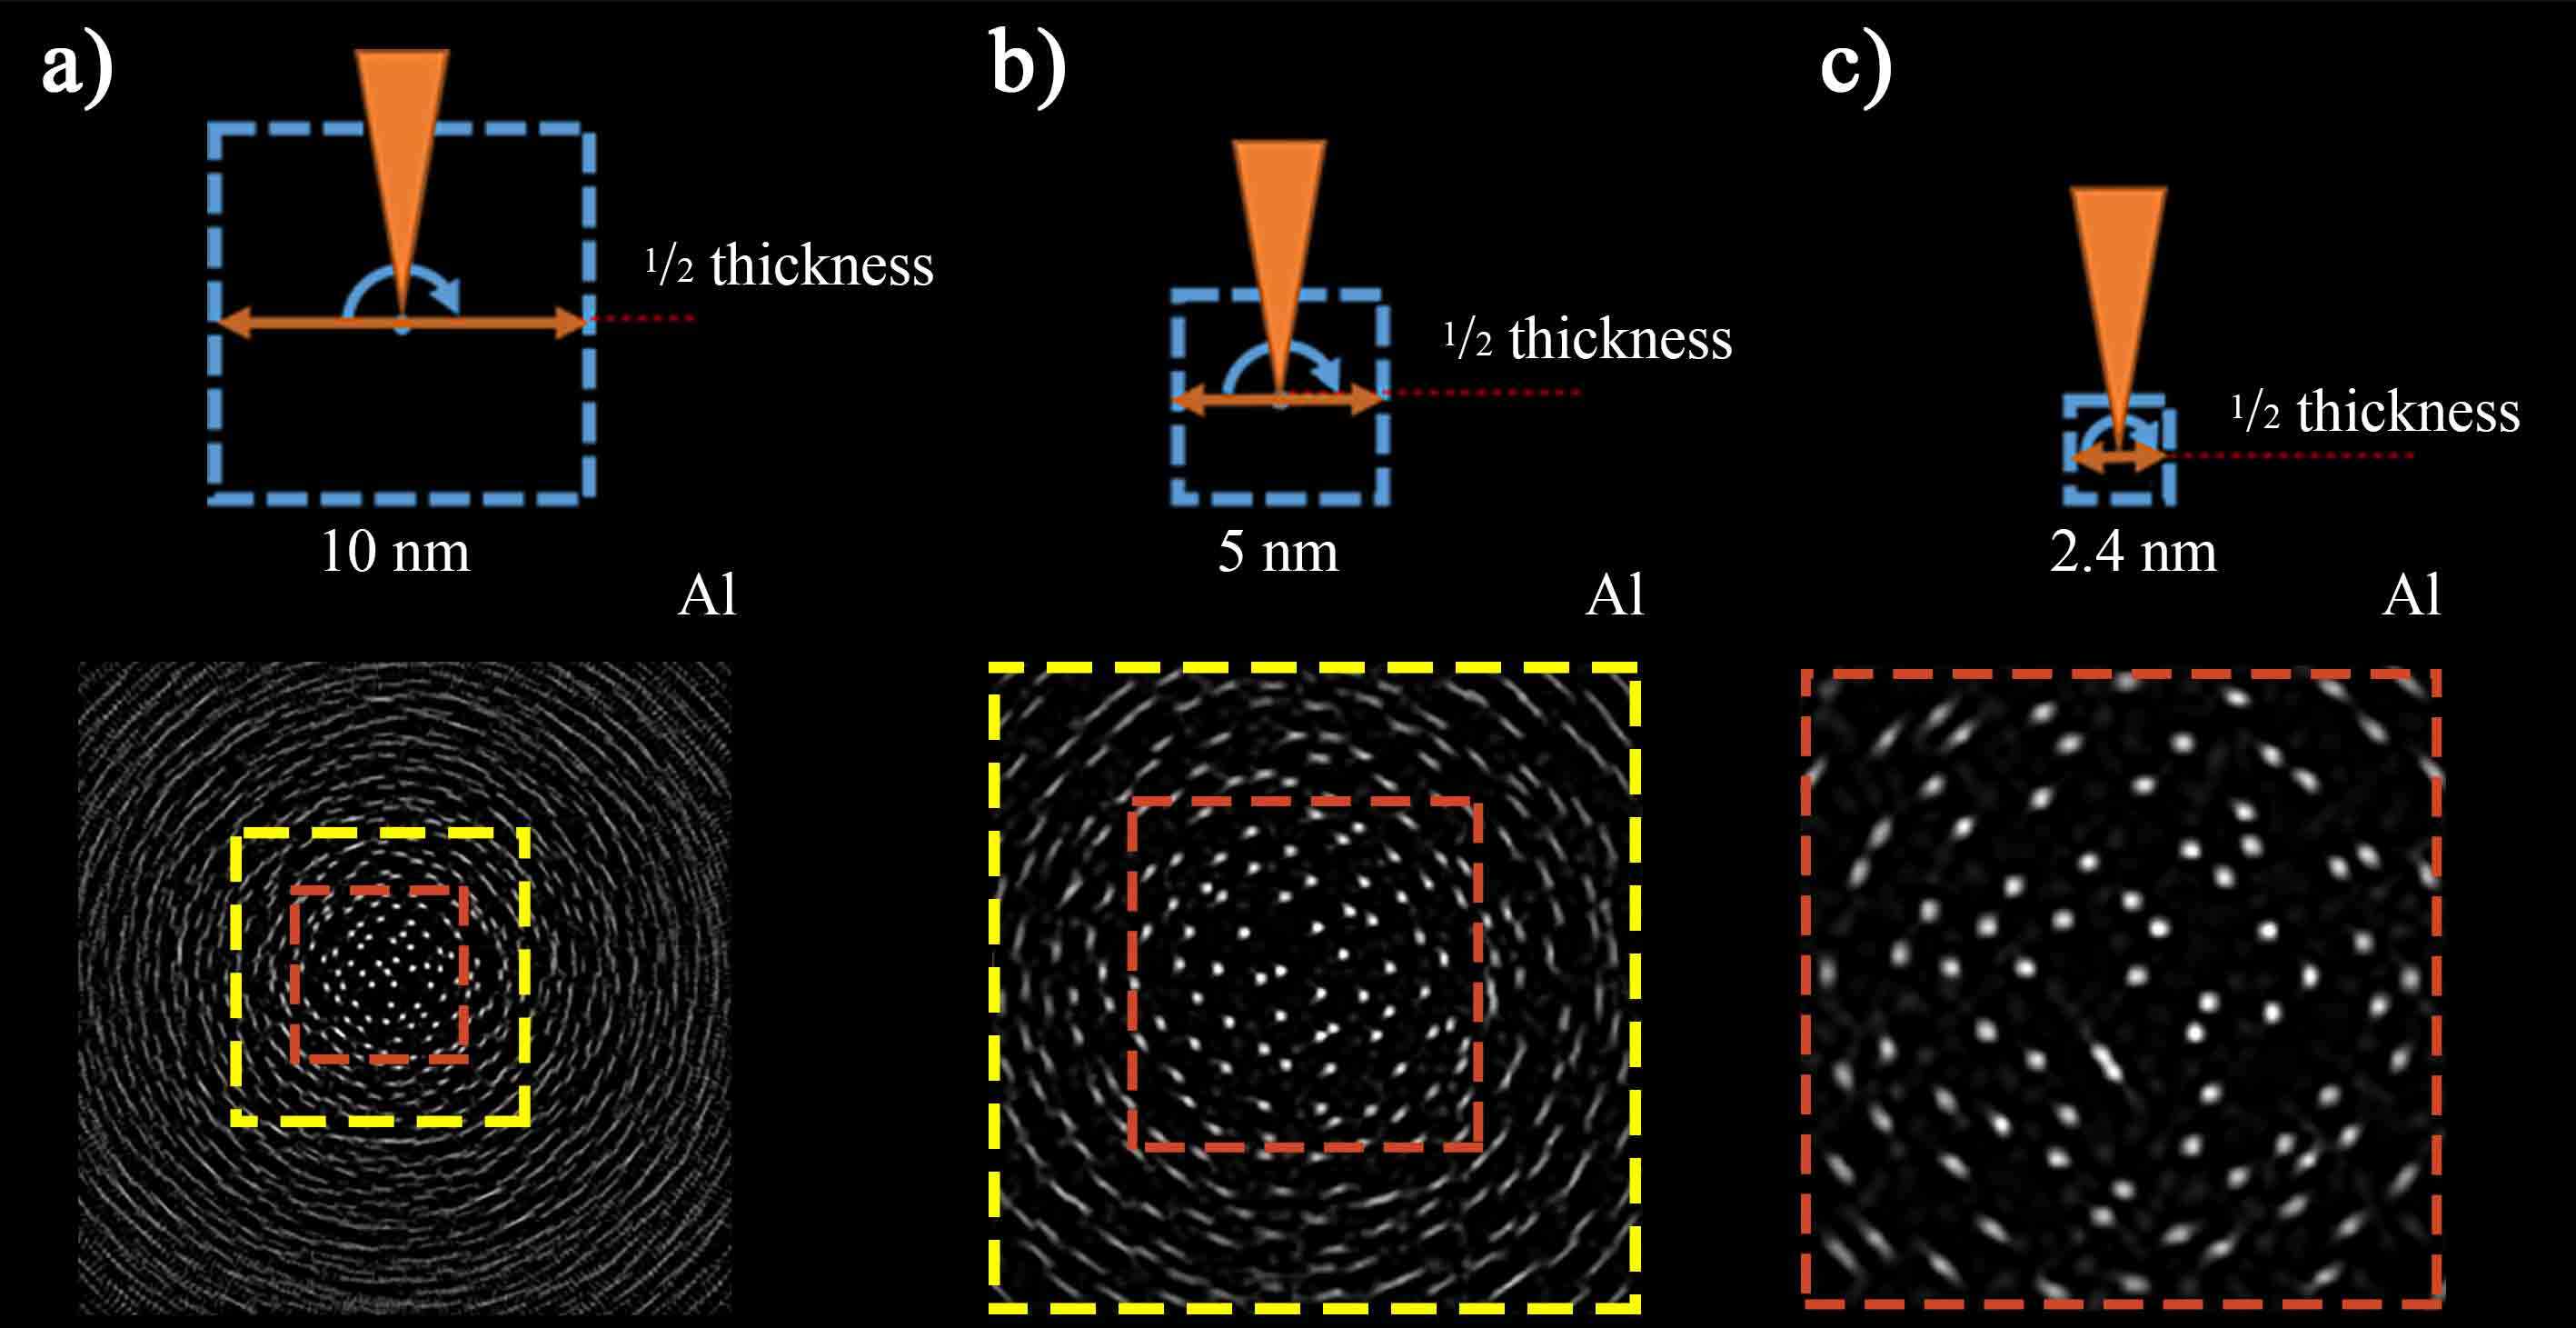
\includegraphics[width=0.85\textwidth]{../4.4/44}
	\caption{不同尺寸模型的重构结果}\label{fig:43}
	\song\tuzhu{a) 10 nm $\times$ 10 nm $\times$ 2.4 nm;b) 5 nm $\times$ 5 nm $\times$ 2.4 nm;c) 2.4 nm $\times$ 2.4 nm $\times$ 2.4 nm;电子束会聚半角均为 50 mrad,加速电压是 200 kV。电子束斑被聚焦到样品厚度 1/2 的深度位置。图中红色虚线框边长的实际长度是 2.4 nm,黄色虚线框边长的实际长度是 5 nm}
\end{figure}





\begin{figure}[H]
	\vspace{\baselineskip}
	\centering
	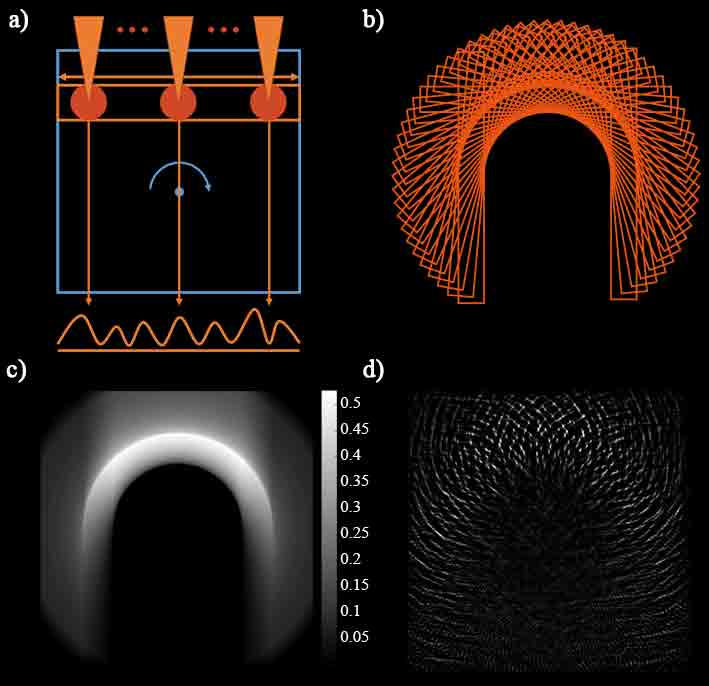
\includegraphics[width=0.9\textwidth]{../4.3/43}
	\caption{电子束景深小于样品厚度时,HAADF-STEM 倾转系列三维重构原理示意图}\label{fig:44}
	\song\tuzhu{a) HAADF-STEM 成像过程,图中橙色圆圈表示景深;b) 倾转系列像中的样品信息在重构时的分布示意图;c) 图 b 对应的信息恢复率;d) 对应情况的模拟重构结果}
\end{figure}

对上述重构结果的解释如图 3.5 所示。图 3.5a 描述了 STEM 图像的形成过程,当电子束斑(即横向分辨率和纵向景深)小于样品厚度时,它在样品中的实际影响范围有限,只能携带样品的局部结构信息,最终形成的扫描图像,仅具有样品中某一深度范围内(橙色矩形框所示)的结构信息,即形成光学层析。该成像模式下产生的倾转系列像,在三维重构的过程,其中包含的样品信息将以如图 3.5b 所示的模式被用于重构。正确的三维重构,需要将每一个倾转角下的图像所携带的样品的结构信息,通过反拉登变换,正确地恢复到对应位置,然后把这些信息叠加。但按照图 3.5b 中的信息恢复方式,样品的信息并不能被完全正确地恢复至正确位置,信息恢复率如图 3.5c 所示。图 3.5d 是该模式下的某一模拟重构图像,对比图 3.5c 和图 3.5d 可知,信息恢复率高的位置,原子可以被正确地重构出来。在图 3.5c 中,信息恢复率最高是 55\%,这说明该位置的重构结果,在 180° 全角度倾转的重构条件下,其实际有效信息仅有 -50° 至 50°,存在严重的缺失锥现象,只是当重构的对象原子的形状为小圆点时,缺失锥效应不严重。进一步容易知道,信息恢复率和入射电子束聚焦的位置与倾转轴之间的相对位置具有直接关系。当电子束聚焦的位置与倾转轴重合时,如图 3.3b 和图 3.4a-c 中的情形,其重构时的信息覆盖率最高,中心可达 100\%。当电子束聚焦点远离倾转轴时,重构的质量会变差。另外,显然的是,正确重构的区域根据电子束聚焦的深度变化,且该区域的尺寸直接决定于电子束的景深。



\subsection{提前聚焦现象}
电子束在不同材料中的传播情况是不同的。图 3.6 对比了将会聚半角均为 $\textnormal{50 mrad}$,加速电压为 200 kV 的电子束,分别聚焦到尺寸均为 10 nm $\times$ 10 nm $\times$ $2.4\textnormal{ nm}$ 的铝和金原子(原子序数分别为 13 和 79)模型的 1/2 深度时的重构结果。图 3.6b 是图 3.6a 和 c 中心区域的放大图,其中红色圆点标出了两图中相同原子所在的位置。仔细观察和对比,可以发现,在相同成像条件下,不同元素的原子模型中可以正确重构的区域的尺寸是相近的。不过,这两个区域位置并不重合。在图 3.6b 铝原子模型的重构图中,红色圆点标记的下方仍然存在清晰重构的原子。但图 3.6b 金原子模型的重构图中,红色圆点标记的下方的原子并没有被清晰地重构,但是上方却有更多被清晰重构的原子。直接对比图 3.6a 和 c 也能发现,图 3.6a 中正确重构的区域在图像的中心,而图 3.6c 中正确重构的区域相对偏上。这相当于在图 3.6b 中,电子束斑并不是会聚于样品的中心,而是在上方提前聚焦了。  

\begin{figure}[H]
	\vspace{\baselineskip}
	\centering
	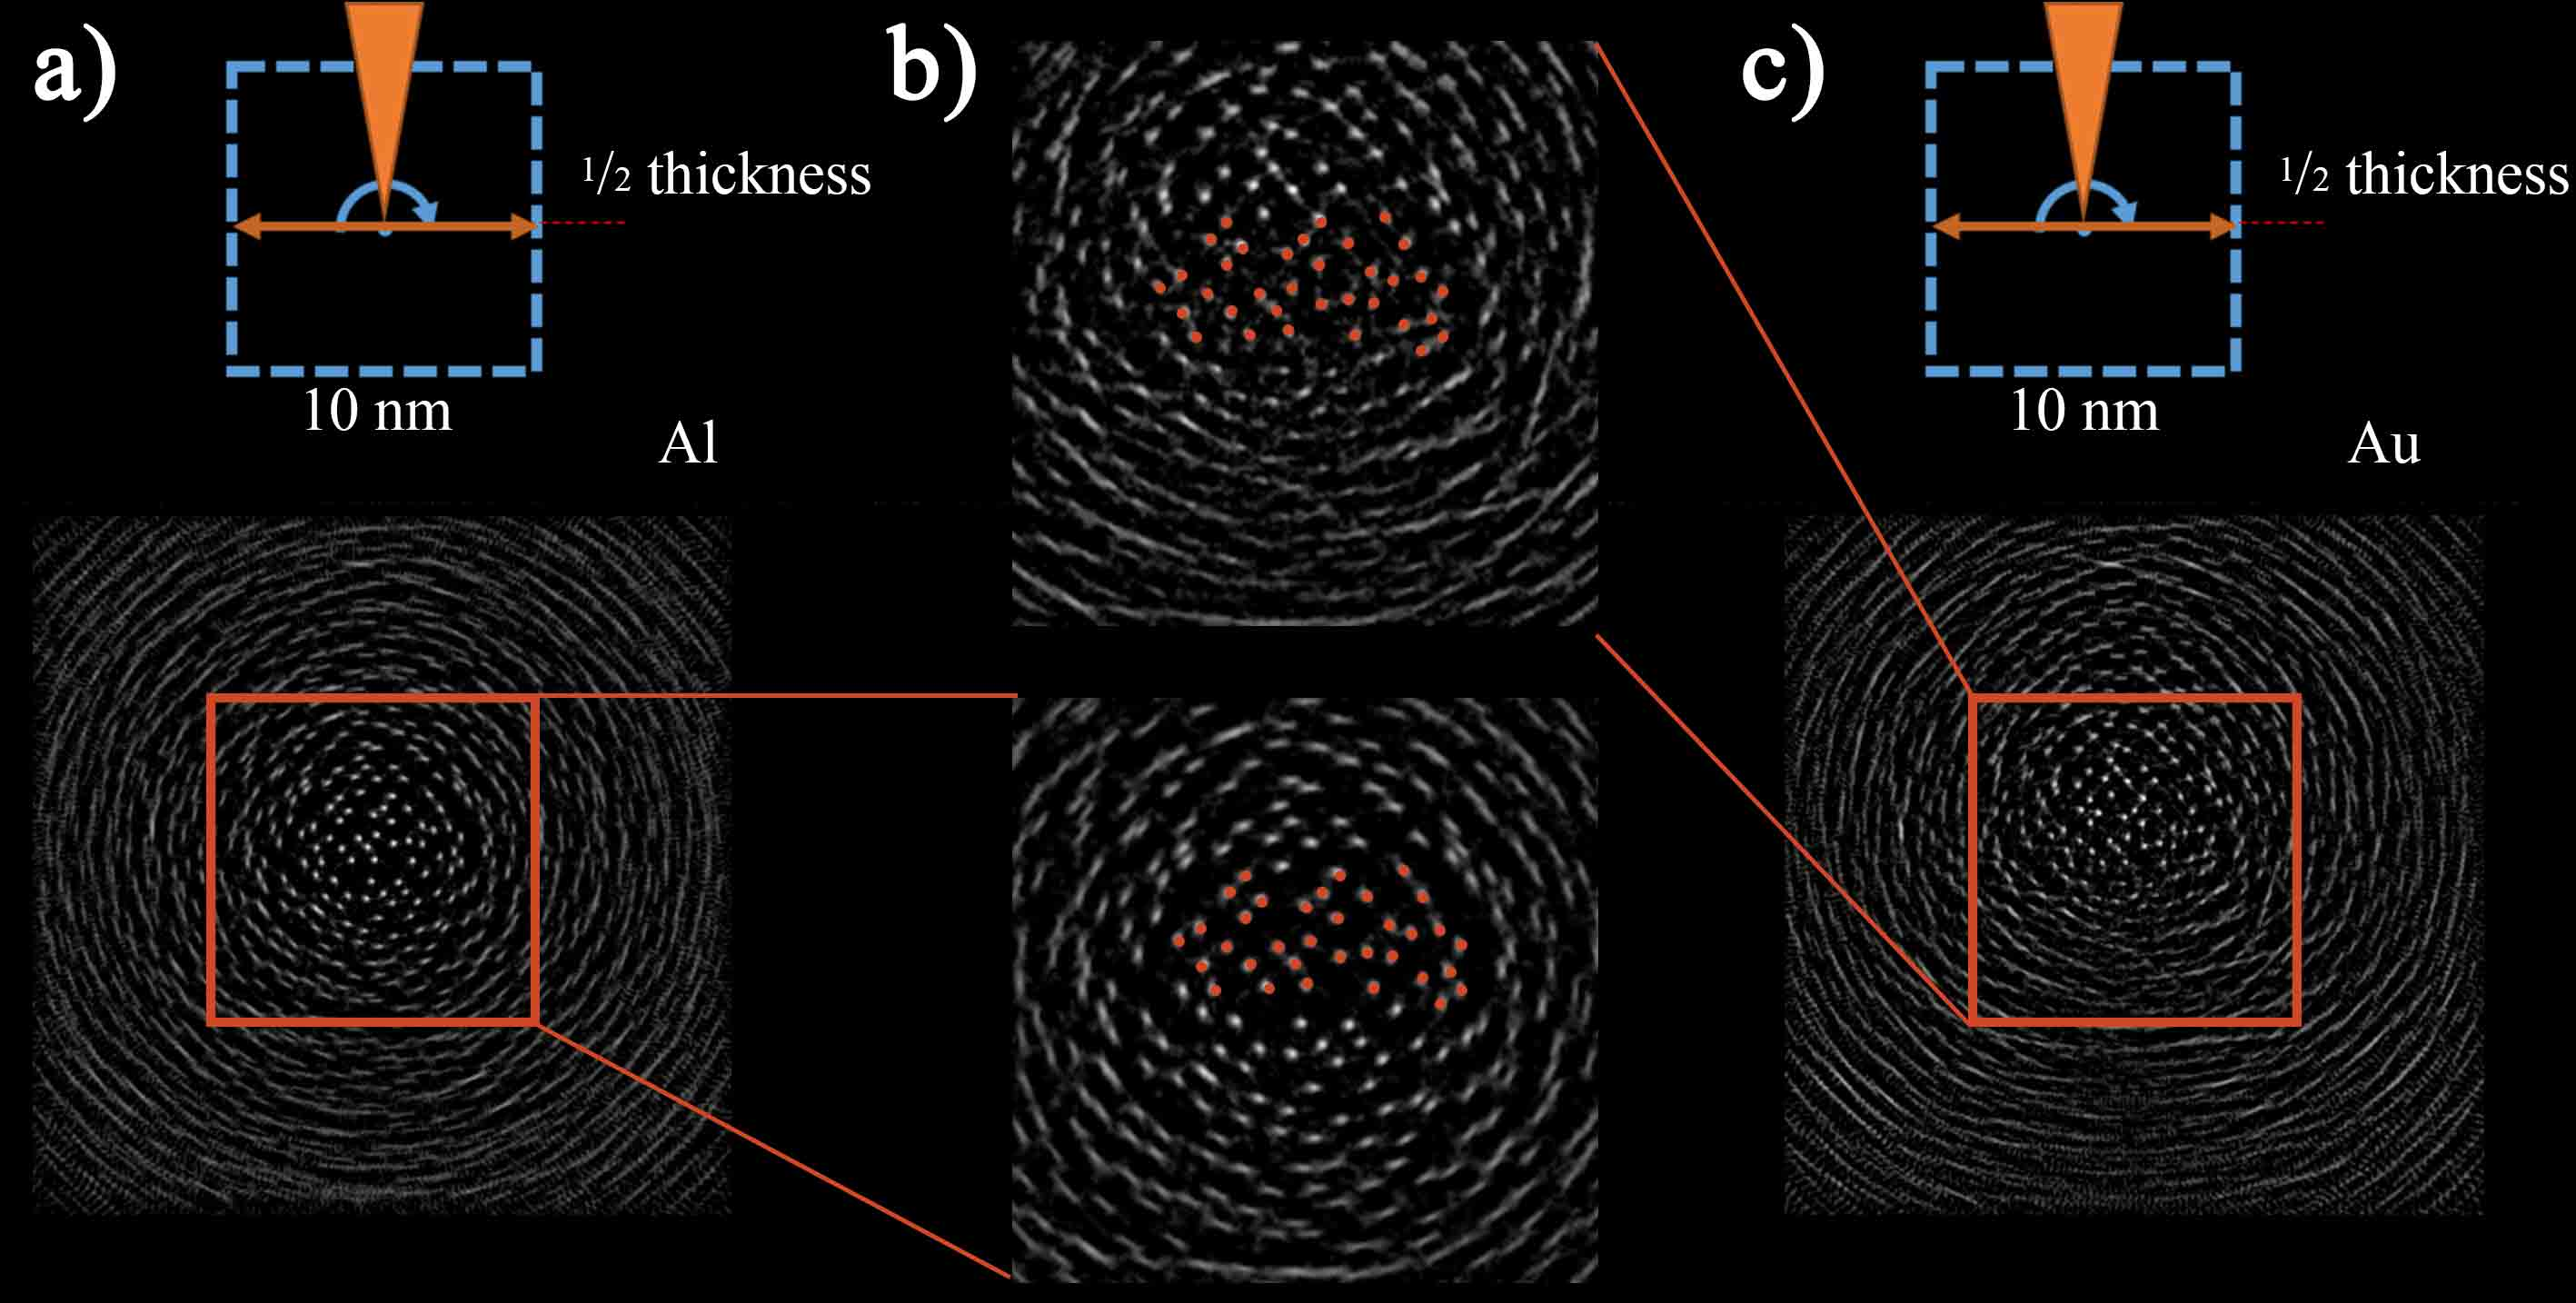
\includegraphics[width=0.9\textwidth]{../4.6/46}
	\caption{提前聚焦现象示意图}\label{fig:45}
	\song\tuzhu{a) 尺寸为 10 nm $\times$ 10 nm $\times$ 2.4 nm 的铝原子模型的重构结果;b) 图 a 和 c 的中心区域放大图,其中红色的圆点表示两个区域中相同的正确重构的原子位置;c) 尺寸为 10 nm $\times$ 10 nm $\times$ 2.4 nm 的金原子模型的重构结果;在模拟中,会聚半角均为 50 mrad,加速电压是 200 kV。电子束斑均被聚焦到样品厚度 1/2 的深度位置}
\end{figure}


图 3.7 更进一步探究了会聚半角和加速电压对提前聚焦现象的影响。图 3.7a-c 对应的参数分别为会聚半角 50 mrad,加速电压 200 kV;会聚半角 30 mrad,加速电压 200 kV;会聚半角 50 mrad,加速电压 100 kV。它们对应的景深分别为 $1。0\sim3.5$ nm,$2.8\sim9.8$ nm,$1.5\sim5.1$ nm。通过对比发现图 3.7b 中正确重构的区域最大,图 3.7a 中正确重构的区域最小,该结果与它们对应的电子束的景深大小相吻合。图 3.7a-c 中正确重构的区域均不在模型的中心处,都发生了提前聚焦的现象,且图 3.7b 中提前聚焦的程度最高。这是因为图 3.7b 对应的电子束的景深最大,能量的集中程度反而最低,因此最容易受到静电势的影响而提前聚焦。

\begin{figure}[htbp]
	\vspace{\baselineskip}
	\centering
	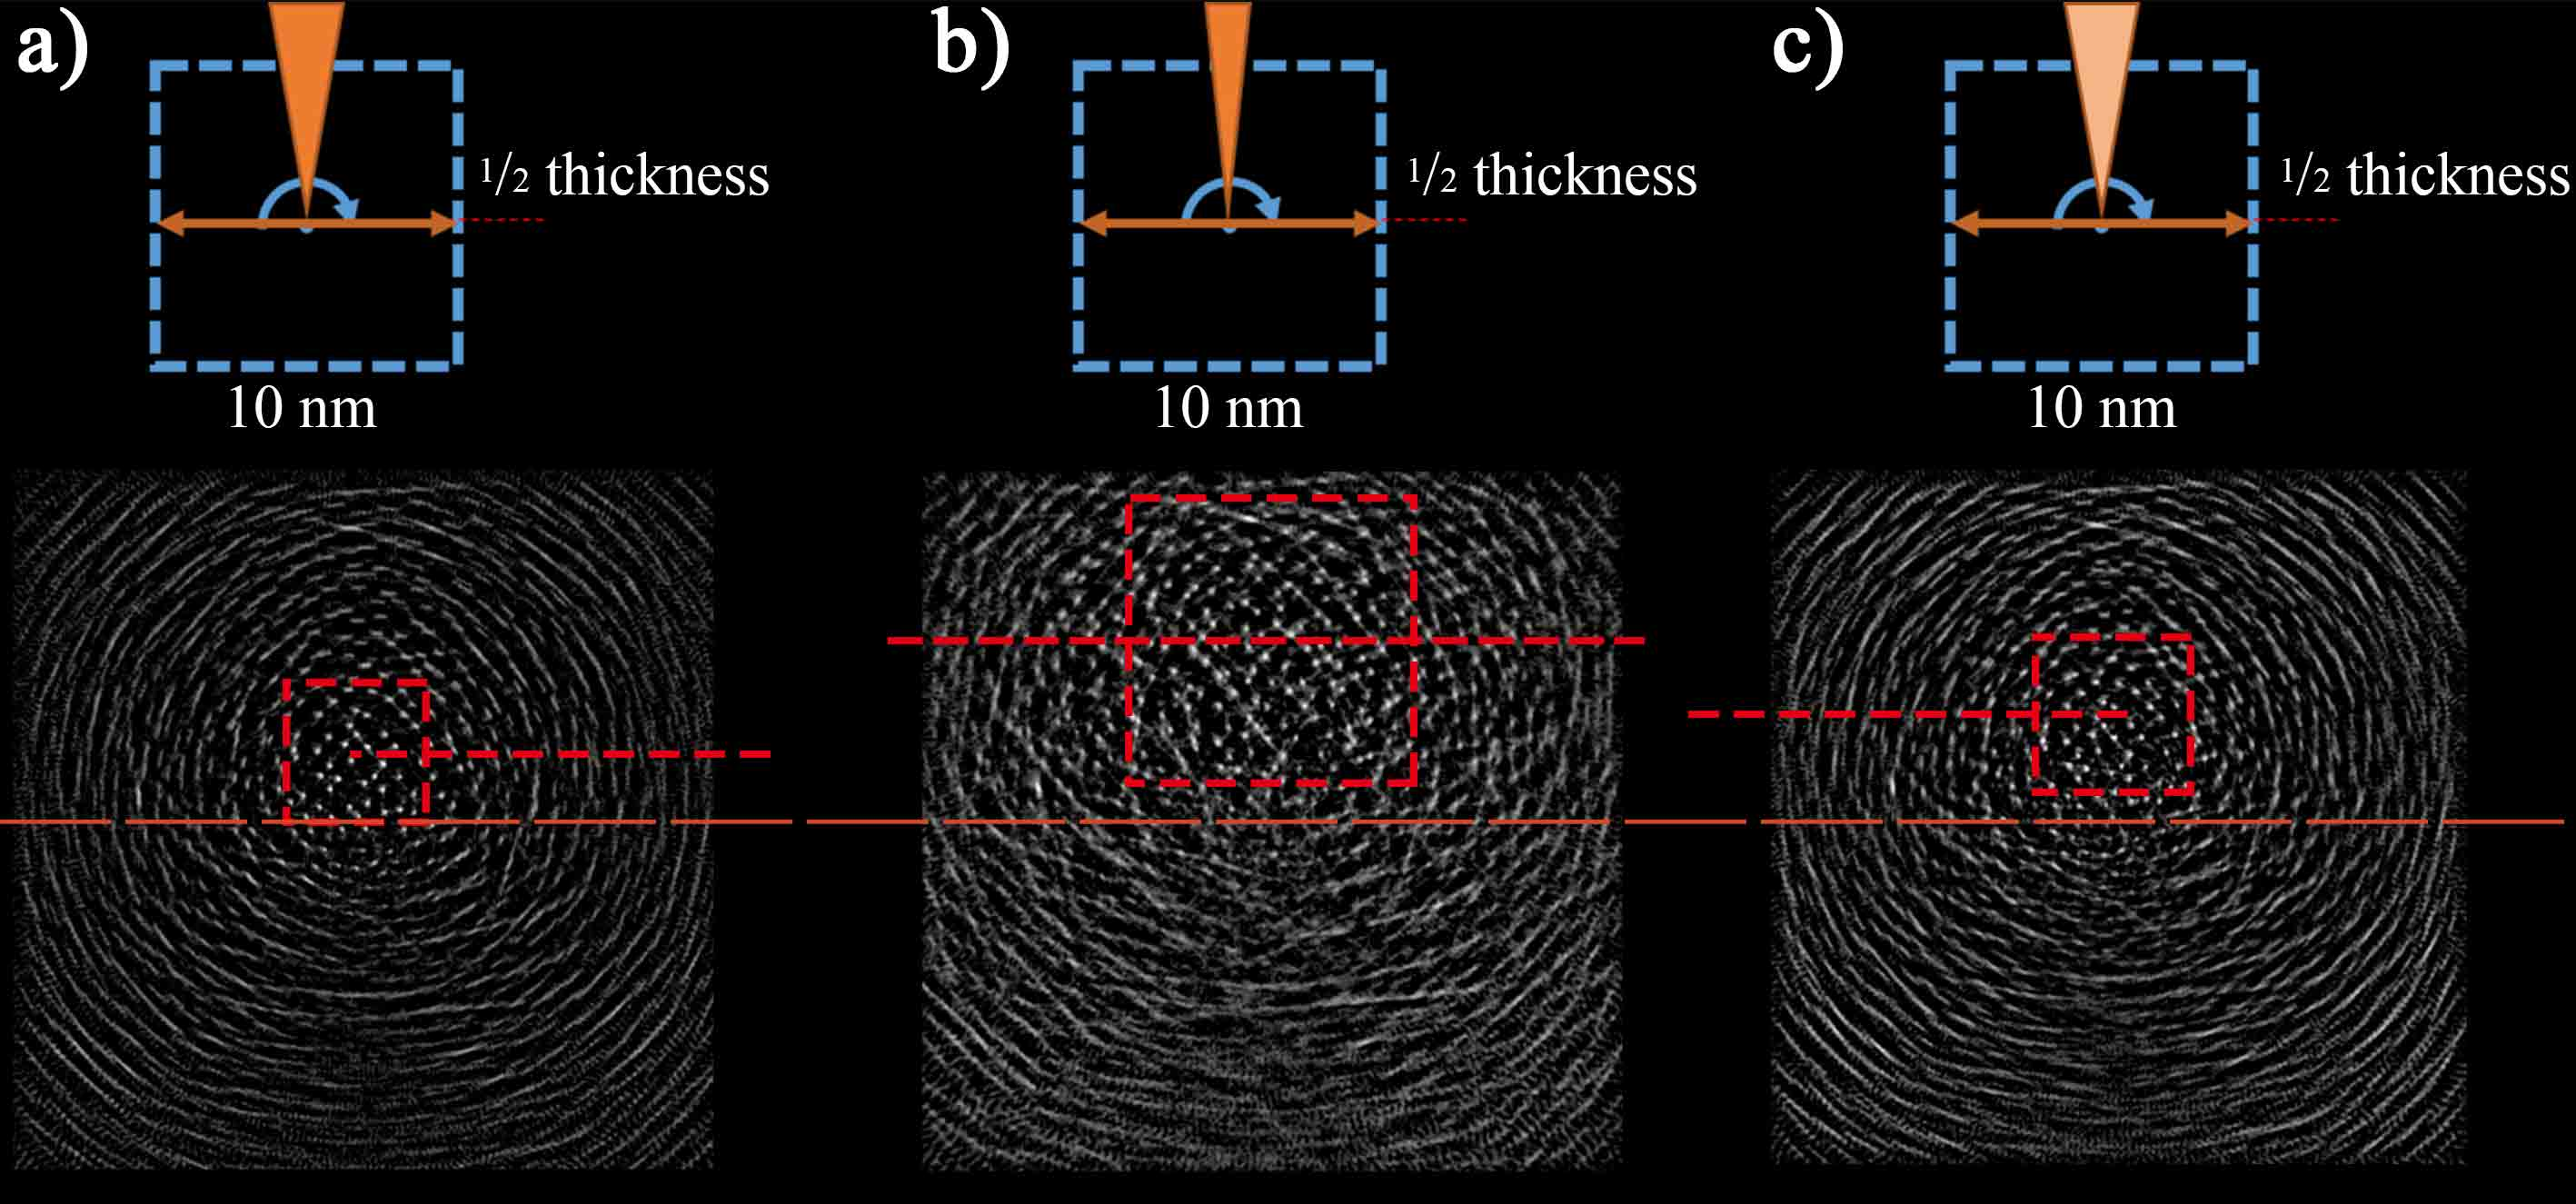
\includegraphics[width=0.9\textwidth]{../4.7/47}
	\caption{不同参数的会聚束引起的提前聚焦现象}\label{fig:46}
	\song\tuzhu{尺寸为 10 nm $\times$ 10 nm $\times$ 2.4 nm 的金原子模型的重构结果:a) 会聚半角均为 50 mrad,加速电压是 200 kV;b) 会聚半角均为 30 mrad,加速电压是 200 kV;c) 会聚半角均为 50 mrad,加速电压是 100 kV;电子束斑均被聚焦到样品厚度 1/2 的深度位置}
\end{figure}

为了加深对这种现象的理解,本研究对电子束斑在不同情况下的强度分布进行了模拟。图 3.8 展示了不同成像参数、不同原子元素下,将电子束名义上聚焦至倾转 30° 的 10 nm $\times$ 10 nm $\times$ 2.4 nm 原子模型的中心(原点 (0, 0))时,电子束斑的实际强度分布情况。在铝原子模型,即图 3.8a 和 c 中,电子束的束斑关于原点呈中心对称分布,其形状与真空中的理想束斑相近。这是因为铝原子的静电势较弱,对电子束斑的强度分布影响较小。因此,在图 3.6a 中没有发现提前聚焦的现象。反观$\textnormal{图 3.8b 和 d}$,两图中的电子束斑的强度分布都发生了扭曲,向上方偏离,这说明金原子的静电势对电子束斑的强度分布产生了较大的影响,最终导致提前聚焦的现象,这与图 3.6c 的结果吻合。对比图 3.8b 和 d 可以发现,当会聚半角为 30 mrad,即电子束会聚程度较低时,束斑的强度中心向上偏离的程度更大,这与图 3.7a 和 b 的结果一致。


\begin{figure}[H]
	\vspace{\baselineskip}
	\centering
	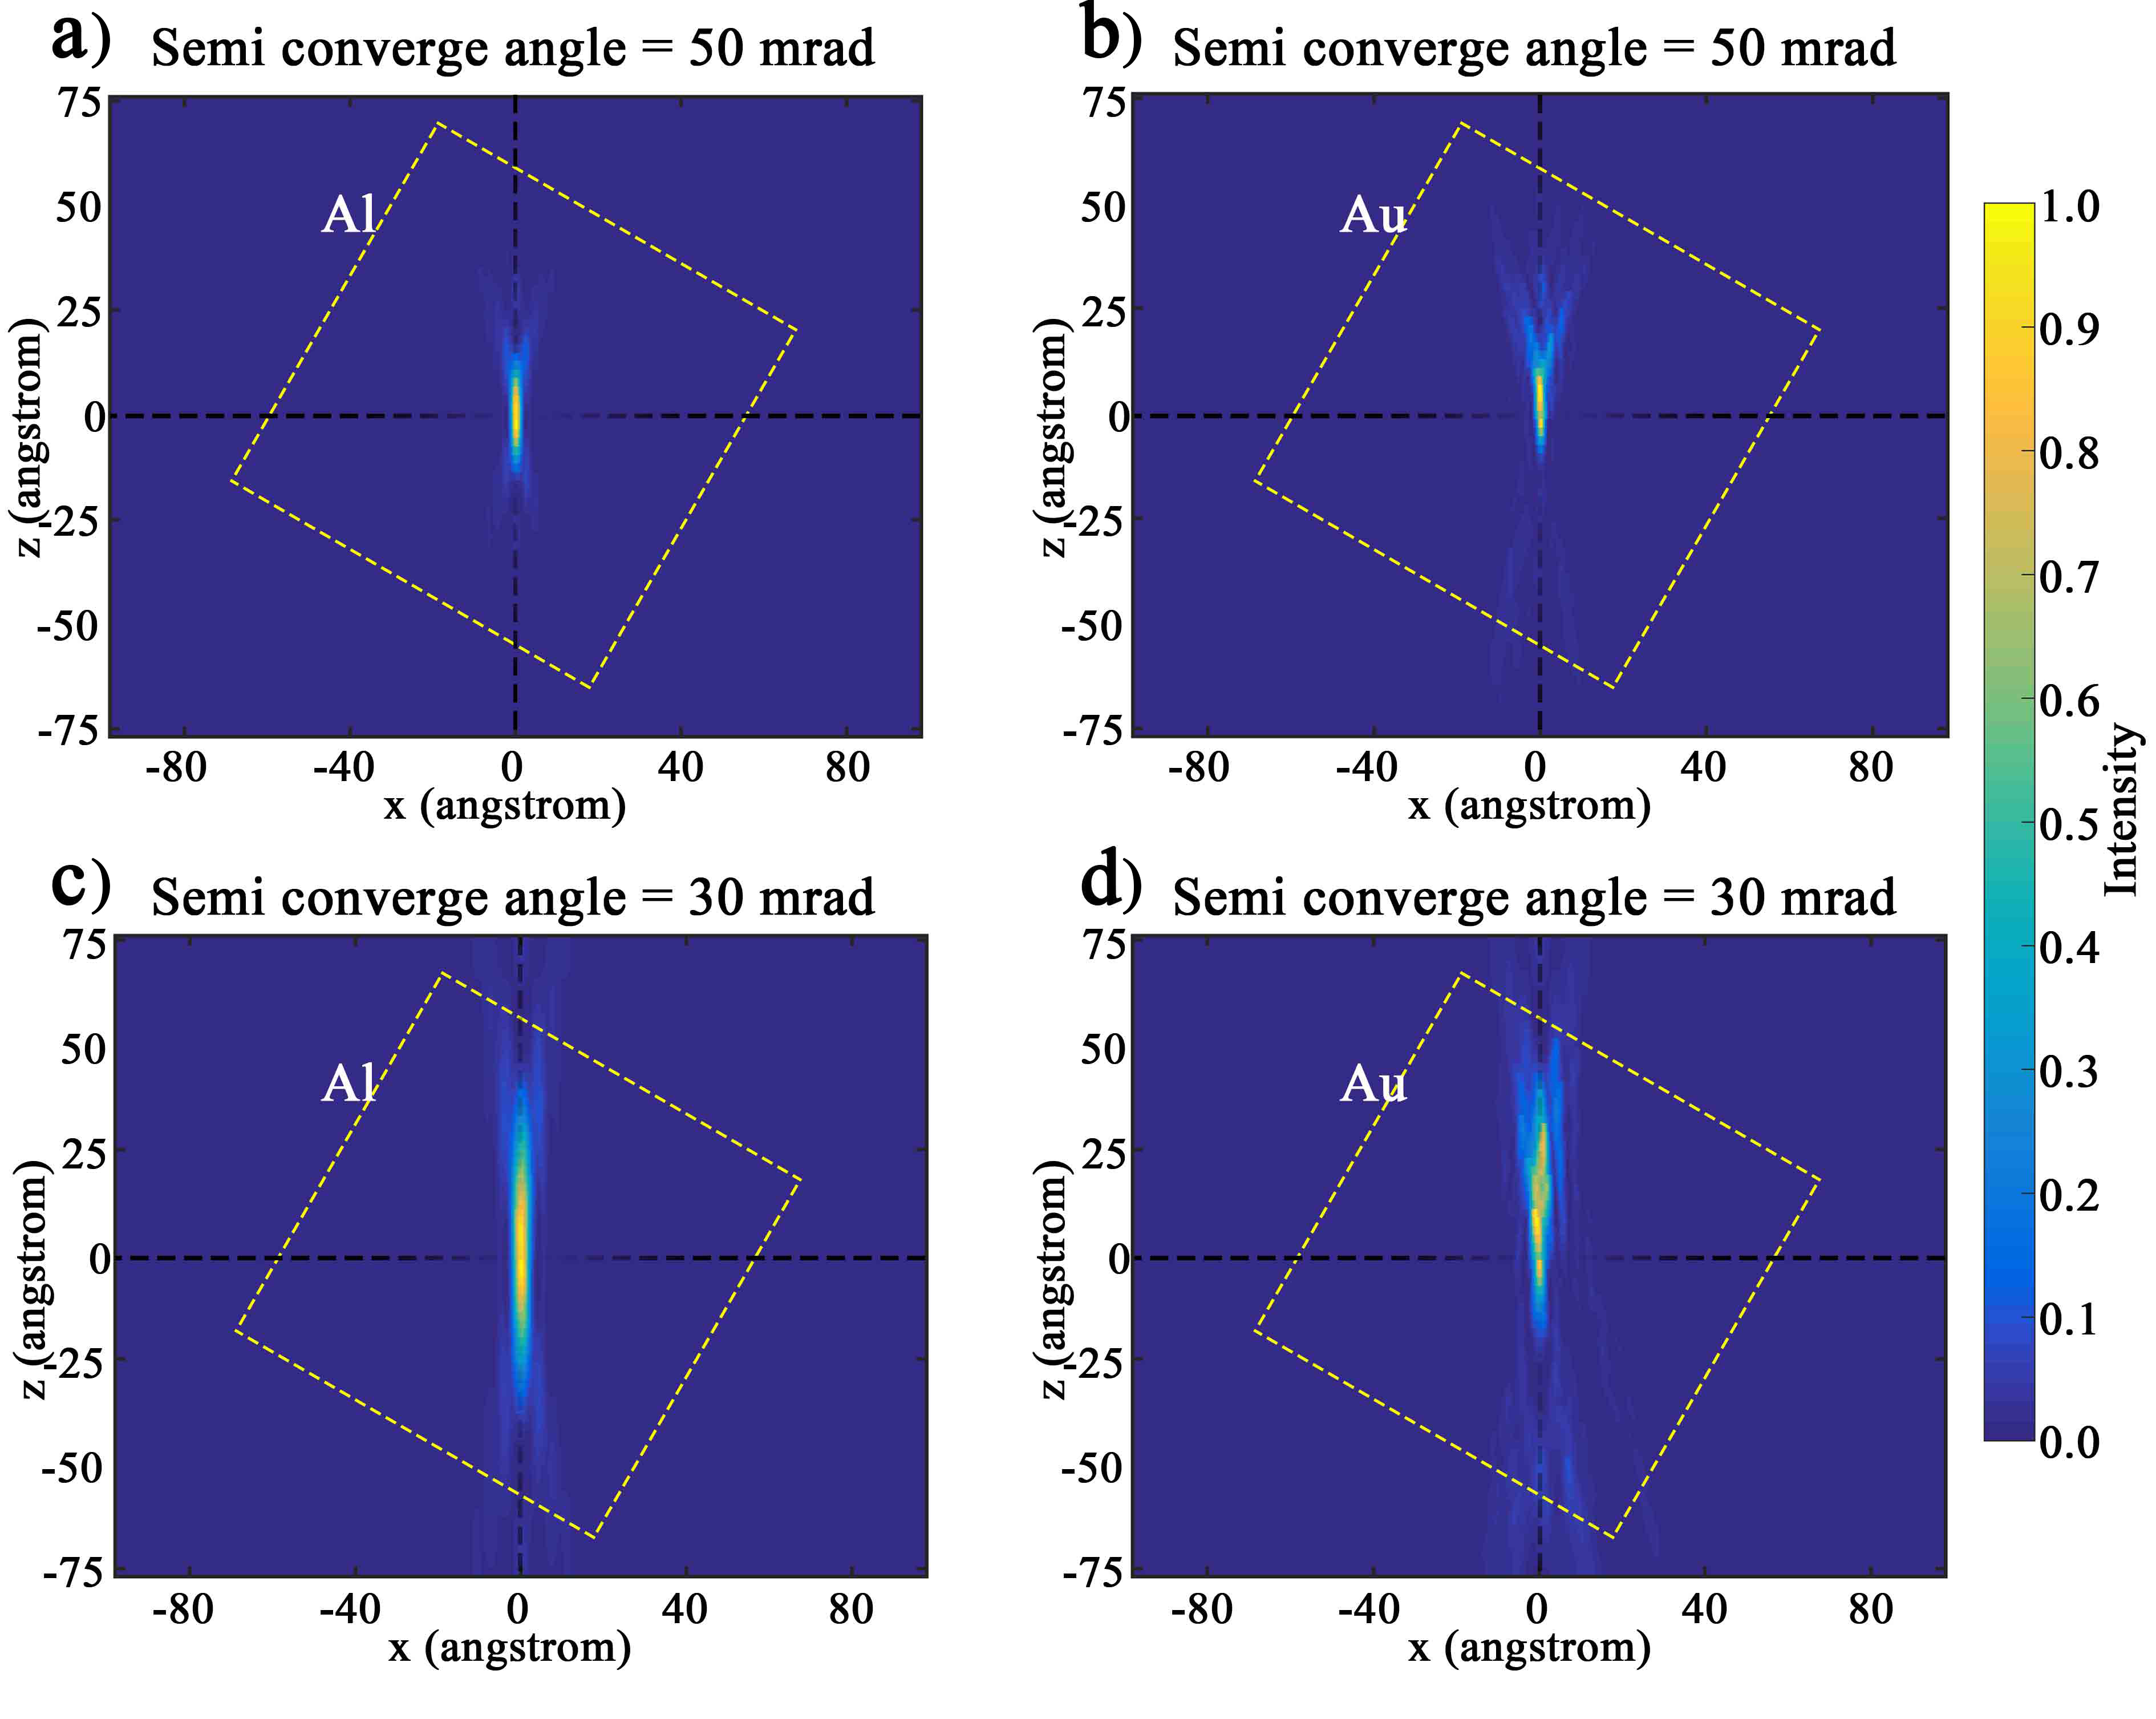
\includegraphics[width=0.9\textwidth]{../4.10/410}
	\caption{电子束聚焦至 10 nm $\times$ 10 nm $\times$ 2.4 nm 的原子模型中心时,电子束斑的强度分布图}\label{fig:47}
	\song\tuzhu{a) 会聚半角为 50 mrad,模型中的原子是铝原子;b) 会聚半角为 50°,模型中的原子是金原子;c) 会聚半角为 30°,模型中的原子是铝原子;d) 会聚半角为 30 mrad,模型中的原子是金原子;加速电压均为 200 kV,模型倾转 30°,原点 (0,0) 是电子束的名义聚焦位置,黄色虚线框表示模型的边缘}
\end{figure}
\subsection{影响分辨率的因素}
STEM 中电子束的强度分布是决定最终三维重构分辨率的重要因素。$\textnormal{图 3.9a 和 c}$ 比较了在将两个不同条件的电子束会聚至 10 nm $\times$ 10 nm $\times$ 2.4 nm 的金原子模型的 1/2 深度时的重构结果,其中电子束的加速电压均为 200 kV。图 3.9a 对应的电子束的会聚半角为 10 mrad,与普通非球差校正电镜(Cs = 1.2 mm)的最优参数相当,其横向分辨率较低,景深较大。将图 3.9a 与原模型比较可以确定整个块体的重构都是正确的,只是原子图像较模糊。而图 3.9c 对应的电子束的会聚半角为 50 mrad,与球差校正电镜的最优成像参数相当,其横向分辨率高,景深小,所以图 3.9c 中只有局部区域被正确地重构,该区域的原子清晰可辨。该对比直观地反映了分辨率与景深之间存在的矛盾。

图 3.9b 展示了将会聚半角 10 mrad,加速电压 200 kV 的电子束聚焦至 5 nm $\times$ 5 nm $\times$ 2.4 nm 的金原子模型中 1/2 深度时的重构结果。可以发现,尽管电子束的分辨率较低,重构图像中的原子是清晰可分辨的,其与图 3.9a 中的结果大不相同。通过对比图 3.9a 和 b,可以发现,同样的成像参数用于不同厚度的样品的三维重构时,重构结果的分辨率是不同的,样品厚度越小,重构分辨率越高。这个结果符合克劳瑟准则~\cite{Crowther1970},详情可见第 1.3.10 条。

图 3.9d 展示了将会聚半角 10 mrad,加速电压 200 kV 的电子束聚焦至 10 nm $\times$ 10 nm $\times$ 2.4 nm 的铝原子模型中 1/2 深度时的重构结果。在轻元素的模型中,尽管电子束的分辨率较低,整个模型中的原子依然都能被清晰地重构出来。该重构结果与图 3.9a 对比可知,实际样品的元素也会影响三维重构的分辨率,轻元素的样品更容易重构。

\begin{figure}[H]
	\vspace{\baselineskip}
	\centering
	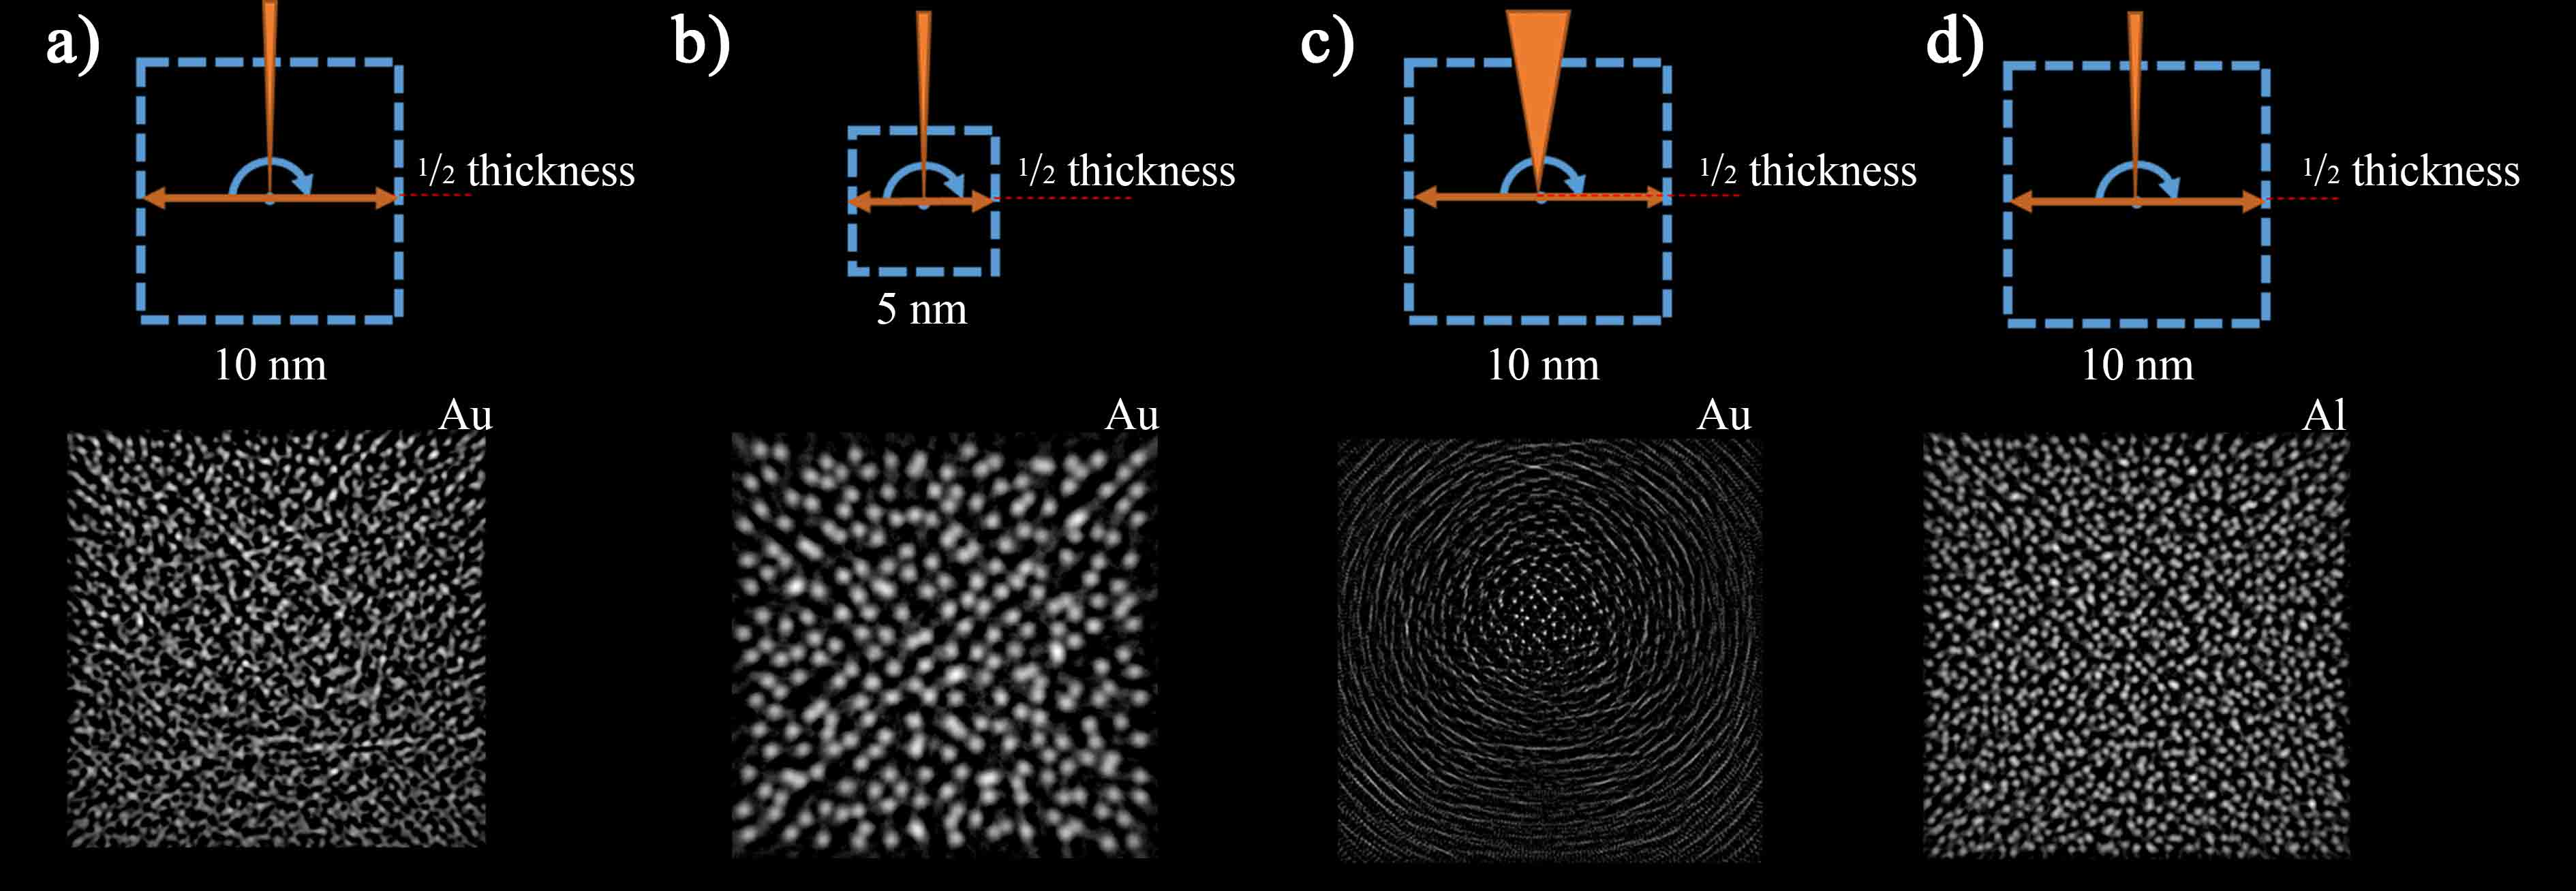
\includegraphics[width=0.85\textwidth]{../4.8/48}
	\caption{影响三维重构的分辨率的因素}\label{fig:48}
	\song\tuzhu{a) 尺寸为 10 nm $\times$ 10 nm $\times$ 2.4 nm 的金原子模型的重构结果。电子束会聚半角为 10 mrad;b) 尺寸为 5 nm $\times$ 5 nm $\times$ 2.4 nm 的金原子模型的重构结果,电子束会聚半角均为 10 mrad;c) 尺寸为 10 nm $\times$ 10 nm $\times$ 2.4 nm 的金原子模型的重构结果,电子束会聚半角均为 50 mrad;d) 尺寸为 的铝原子 $10 \textnormal{ nm}\times10 \textnormal{ nm}\times2.4 \textnormal{ nm}$ 模型的重构结果,电子束会聚半角均为 10 mrad;电子束斑均被聚焦到模型中 1/2 深度,加速电压是 200 kV}
\end{figure}

\section{讨论}
本工作旨在从理论上探究当 STEM 会聚束景深小于样品尺寸时 3DET 重构的可能性,同时揭示其中的特殊现象和规律~\cite{SRH2020}。在理论模拟中,很多现实因素都没有被考虑在内,比如噪音、样品漂移、放大倍数偏离等。会聚束束斑的模拟局限在理想的电镜系统中。比如 R. Xu 等~\cite{Xu2015}成功重构了原子分辨率的尺寸为 10 nm 的钨针尖,但是他们使用的会聚束束斑的会聚半角是 30 mrad,加速电压为 300 kV,其理论景深根据公式(3.3)只有 $1.3\sim4.5$ nm。所以,实际电镜中会聚束的景深,不能简单的根据现有的公式计算得出。



一般情况下,使用低分辨率及低放大倍数的 STEM 图像重构样品的外形时,只要求图像的强度与样品的厚度呈线性关系。然而,原子分辨率的三维重构对 STEM 图像与样品之间的线性关系的要求无疑更为严格。因为STEM 图像实际反映了原子静电势对电子的散射能力,当重构样品中的原子时,实际重构的是原子的静电势分布,所以原子分辨率 3DET 的关键是原子的静电势信息能够线性地被电子束携带并被探测器接收。本章的模拟与重构结果可以反向证明,当 STEM 会聚束束斑的景深小于样品时,STEM 图像的强度反映了样品某一深度内的原子静电势的投影信息,否则不会出现正确重构的区域。 

\begin{figure}[htbp]
	\vspace{\baselineskip}
	\centering
	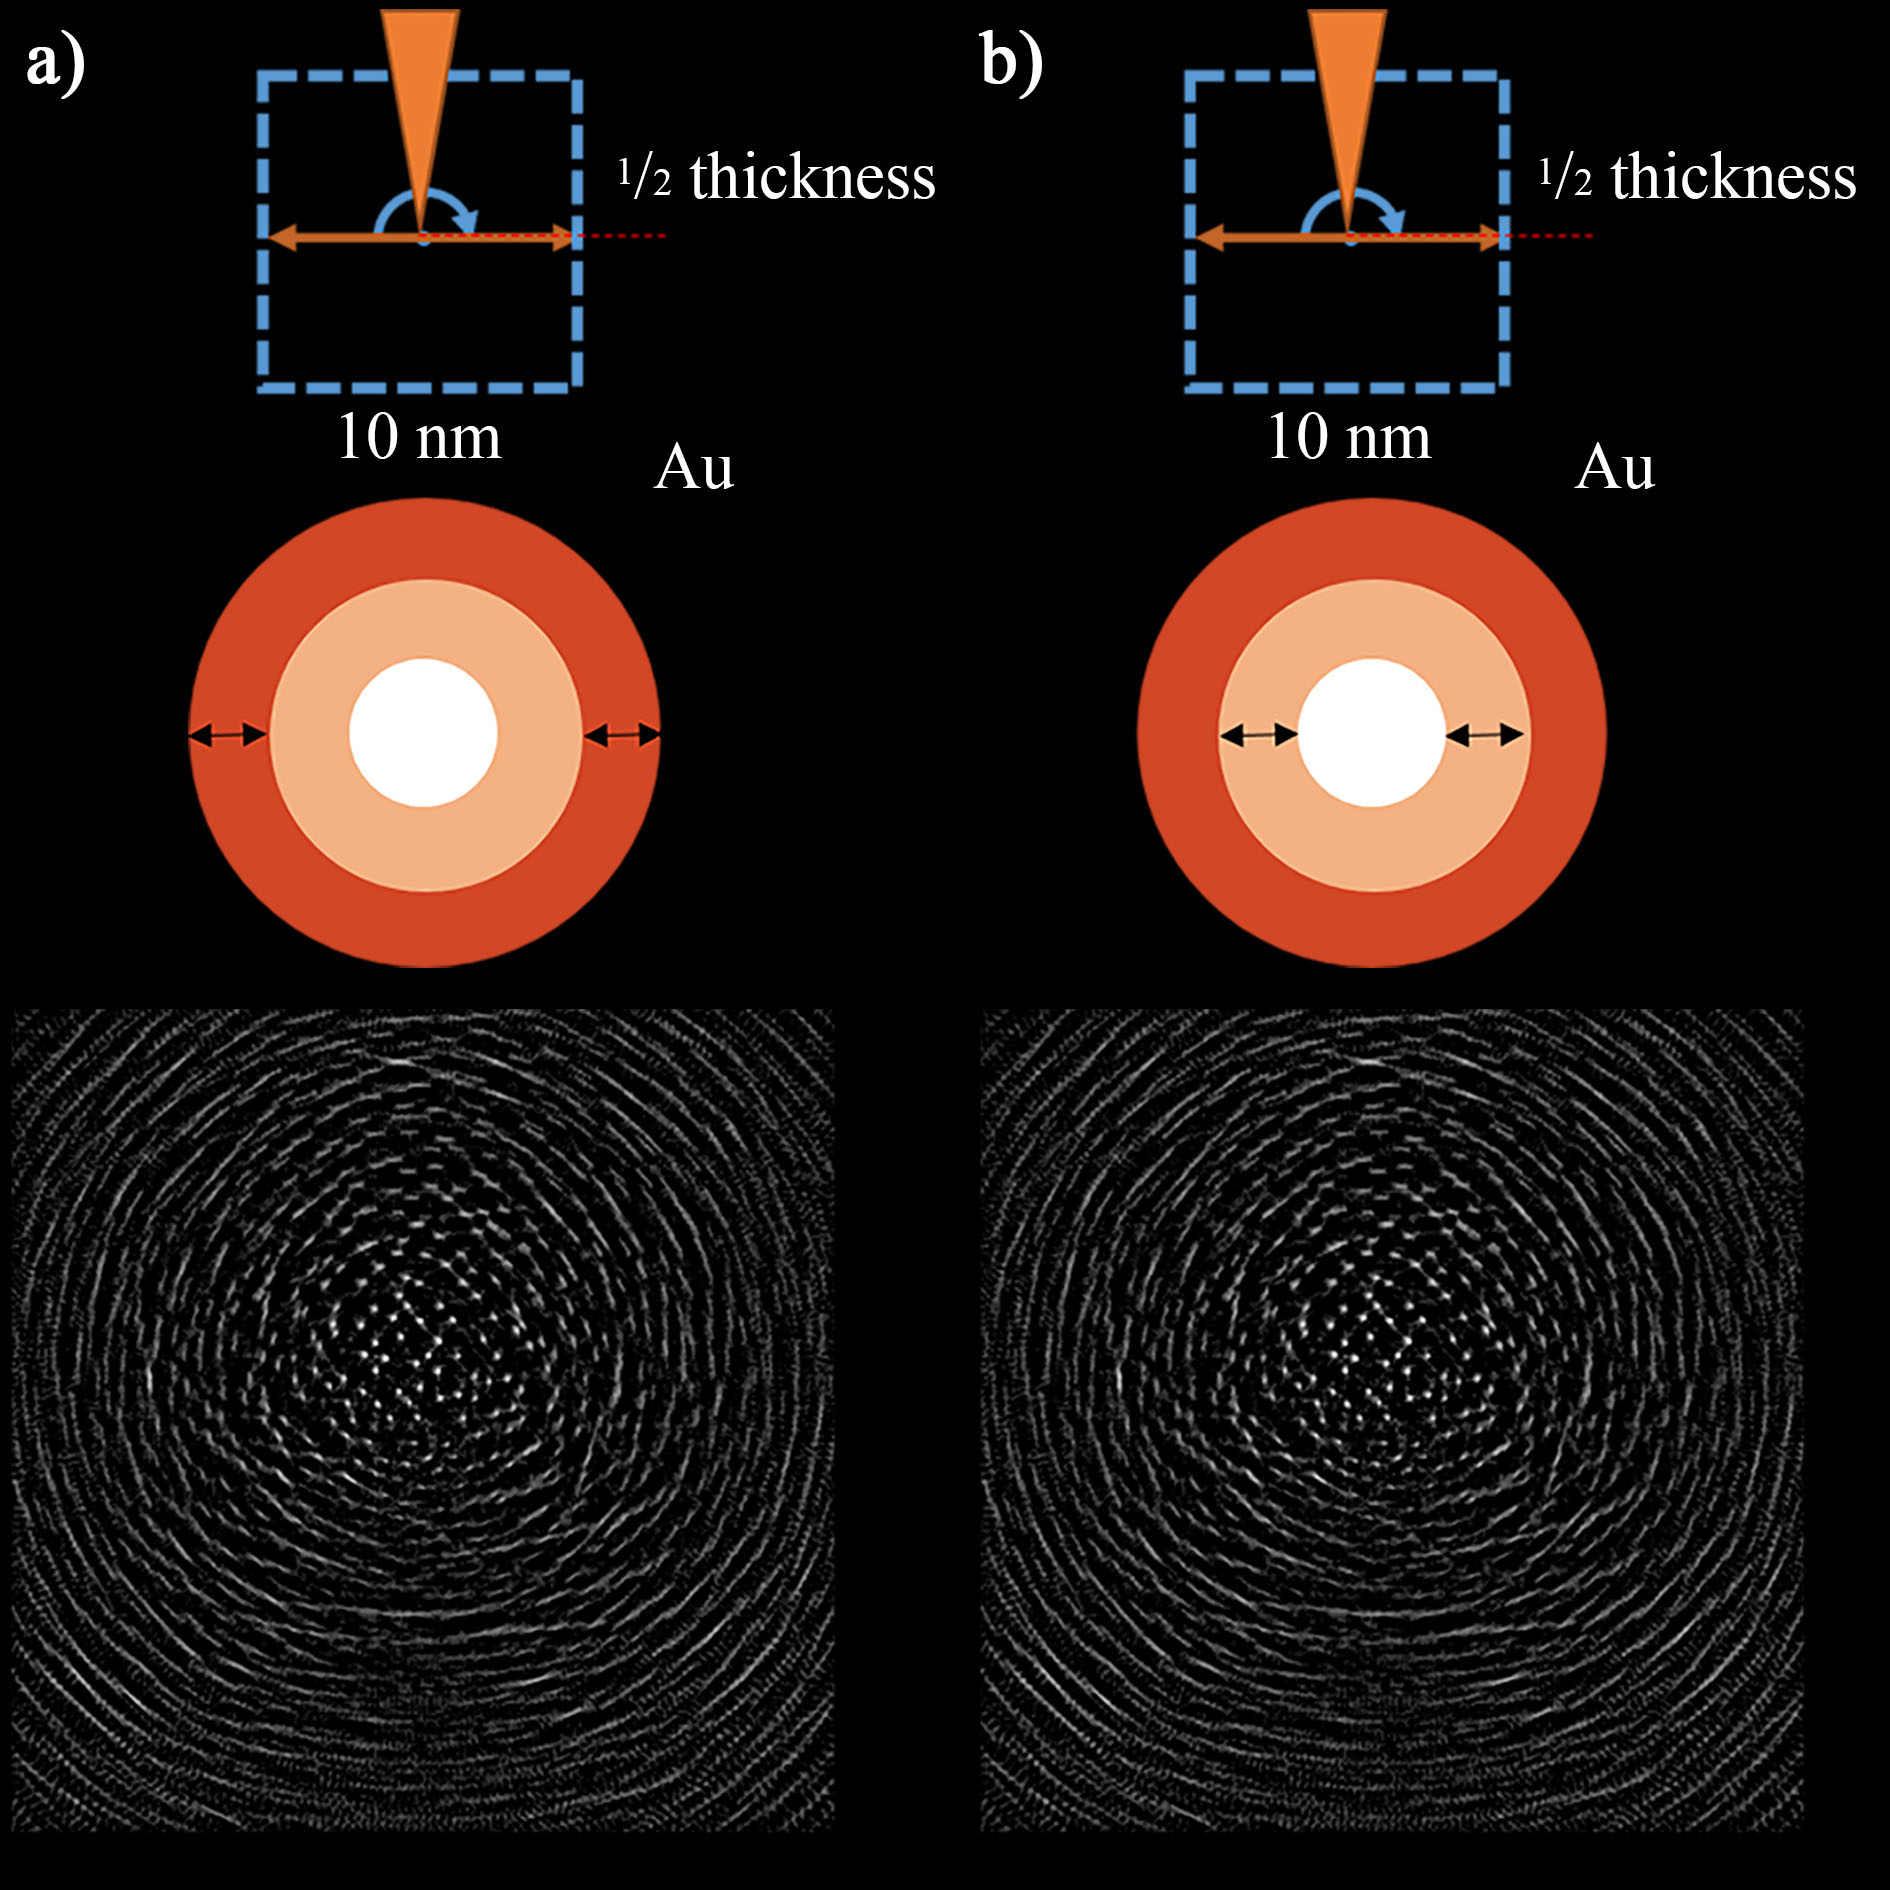
\includegraphics[width=0.9\textwidth]{../4.9/49}
	\caption{尺寸为 10 nm $\times$ 10 nm $\times$ 2.4 nm 的金原子模型在 HAADF 和 ADF 成像模式下的重构结果}\label{fig:49}
	\song\tuzhu{它们的探测器收集角分别为 a) 内角 90 mard,外角 230 mrad,b) 内角 58 mard, 外角 90 mrad;会聚束会聚半角均为 50 mrad,加速电压是 200 kV,会聚束束斑均被会聚到样品厚度 1/2 的深度位置}
\end{figure}

通常认为 HAADF-STEM 图像的的强度与原子序数(Z$^{\sim1.7}$)呈线性关系~\cite{Kubel2005},适合用于 3DET。然而,在 M.C. Scott 等~\cite{Scott2012}和 R. Xu 等~\cite{Xu2015}的研究中使用了 ADF-STEM 倾转系列像成功实现了原子分辨率的三维重构。目前并没有理论能够解释 ADF-STEM 图像与样品之间存在投影关系。图 3.10 通过模拟和重构,比较了 HAADF 和 ADF 两种模式下的重构。图 3.10a 中的 STEM 探测器收集角是 90 mrad $\sim$ 230 mrad,图 3.10b 则为 58 mrad $\sim$ 90 mrad。两个重构的结果没有明显的不同,这个结果支持了上述提到的两个原子分辨率三维重构的成果,说明 ADF-STEM 倾转系列像在一定条件下也可以使用于 3DET,尽管其中还有一些理论问题无法被解释清楚。

另外,图 3.11 对比了不同投影数量和角度范围的重构结果。图 3.11a-c 展示了投影角度为全 180°,但投影角度间隔依次为 1°、2°、3° 时的重构结果。可见,当投影数量减少时,图像的噪音增大,有些原子在重构后会“粘连”,产生重构误差。而图 3.11d-f 展示了投影角度范围为 -80°$\sim$+80°、-70°$\sim$+70°、-60°$\sim$+60° 时的重构结果,即缺失锥逐渐严重。此时,重构的质量也会下降。在第 1.3.8 条中已经论述过,缺失锥假象对重构对象的形貌产生影响,并且假象的严重程度与对象的几何形状有关。在本章论述的问题中,重构的对象是呈点状的原子,所以缺失锥假象对重构的影响是有限的,特别是重构的实质信息仅是原子的位置,而非形状。所以,在一般的透射电镜中开展实验时,缺失锥问题不应当是影响重构的重要因素。而投影数量的整体减少,却可与实验噪音共同对重构造成较大影响。


\begin{figure}[htbp]
	\vspace{\baselineskip}
	\centering
	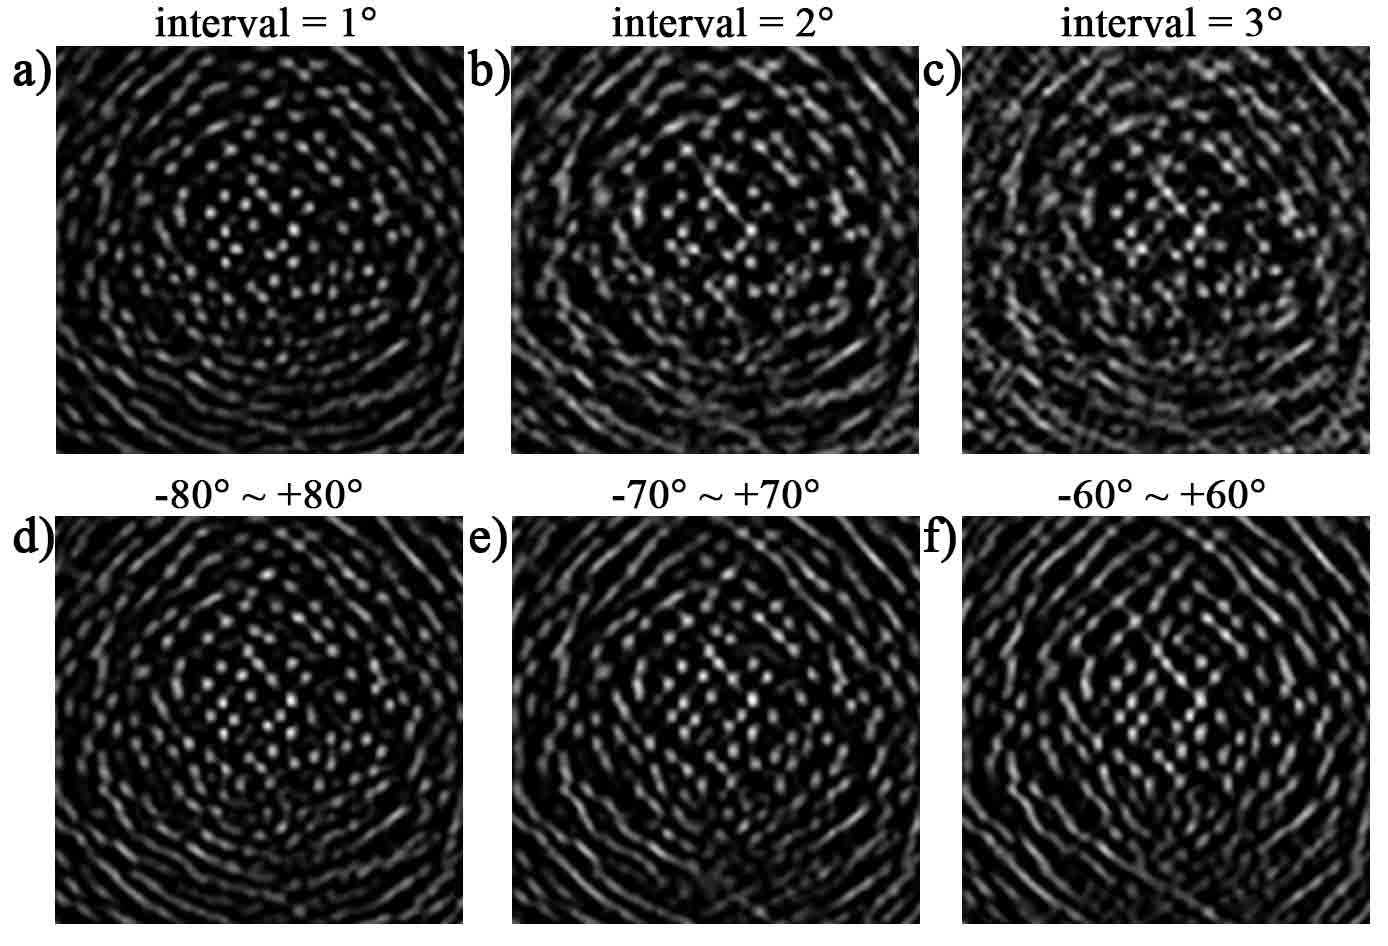
\includegraphics[width=0.9\textwidth]{../4.12/412}
	\caption{投影数量和角度范围对重构的影响}\label{fig:412}
	\song\tuzhu{a) 投影角度是全 180°,角度间隔为 1°;b)  投影角度是全 180°,角度间隔为 2°;c)  投影角度是全 180°,角度间隔为 3°;d)  投影角度是全 -80°$\sim$+80°,角度间隔为 1°;e)  投影角度是全 -70°~+70°,角度间隔为 1°;f)  投影角度是全 -60°~+60°,角度间隔为 1°;模拟参数见图 3.10a,图像取了整图的局部}
\end{figure}


一般的块体材料的三维重构要求 HAADF-STEM 信号反映物体的质厚投影,分辨率较低。HAADF-STEM 信号的本质来源是原子核与电子之间的卢瑟福散射,反映的是原子对电子的散射能力,当讨论问题达到原子分辨率时,我们才逐渐开始讨论到该本质问题,即 HAADF-STEM 的信号强度与这种散射能力之间是否具有良好的线性关系。答案是肯定的,因为 HAADF-STEM 倾转系列像的 tomography 重构结果能够清晰地反映出原子所在的位置,即其重构的原子对电子散射能力在空间中的分布是符合理论预期的。并且,原子的静电势对电子束的汇聚作用在这种情况下也对重构结果产生影响。所以才出现了与重构块体材料时不同的现象。

\section{本章小结}
本章通过理论模拟,探究了景深对三维重构的影响。当 STEM 入射电子束的景深达到纳米尺度,小于样品的厚度时,HAADF-STEM 像仍然可用于 tomography 三维重构。但此时只有样品内部局部区域的原子能被正确地重构。

正确重构的区域位置、厚度以及重构的质量,和入射电子束斑的会聚半角、加速电压、聚焦位置以及其与倾转轴的相对位置有关。保证电子束斑聚焦在与倾转轴同一样品深度,能够最大程度地获得高质量的重构结果。此外,因重元素原子静电势对电子束的作用而带来的提前聚焦现象会干扰对电子束实际束斑位置的精确控制。

要保证足够的三维重构分辨率以分辨原子,不仅要考虑电子束的分辨率与景深,还要考虑样品厚度和样品的元素的影响。尺寸大且内部原子属于重元素的样品较难重构,应尽量选择较大的会聚半角和较高的加速电压;小尺寸、轻元素的样品更容易达到高分辨率的三维重构,所以可以适当选择较小的会聚半角和低加速电压,以获得更大的重构区域。要获得理想的原子分辨率三维重构,需要综合考量分辨率、景深、样品厚度和样品元素等因素对重构结果的影响。

本工作在理论上揭示了原子分辨率的三维重构与一般块体材料的三维重构的差别,对实验具有指导意义。


